
% !TeX program = xelatex

%使用hustthesis这个模板。
% draft版本的正文页包括页眉(“华中科技大学xx学位论文”)、页眉修饰线(双线)、页脚(页码)和页脚修饰线(单线)。
% final版本的正文页不包括页眉、页眉修饰线和页脚修饰线,仅包 含页脚(页码)。如果不指定,默认设置为final。

% degree用来指定论文的种类
% language用来指定论文语言。特别的,如果设定为english-draft,将会剔除论文中的所有中文内容,这有利于在未安装中文字体的环境中使用。如果不指定,默认设置为 chinese。


\documentclass[format=draft,language=chinese,degree=master]{hustthesis}
%\documentclass[format=final,language=chinese,degree=master]{hustthesis}

%使用下面的这两个宏包来生成带书签和超链接的PDF文件。
%\usepackage[bookmarks,bookmarksopen,bookmarksdepth=2]{hyperref}
%\usepackage[pdftex,CJKbookmarks=true,colorlinks=true]{hyperref} %LaTeX Error: Option clash for package hyperref

\stuno{M201672905}
\schoolcode{10487}
\title{基于Vxworks的调试通道的设计与实现}{A design and implementation of debug channel based on Vxworks.}
\author{郑松}{Joe}
\major{计算机应用技术}{Computer Applications Technology}
\supervisor{张杰\hspace{1em}讲师}{Instructor JieZhang}
\date{2018}{3}{26}
%\date{\today}

\zhabstract{数据传输是现代通讯过程中的一个重要环节,在数据的传输过程中,不仅仅要求数据传输的准确率要高,而且要求速度快,连接方便。传统的RS232串口通讯和并口通讯都存在传输速度低,扩展性性差、安装麻烦等缺点,而基于USB接口的数据传输系统能够较好的解决这些问题。目前USB接口以其传输速率高、即插即用、支持热插拔等优点,逐步成为PC机的标准接口。
	
本文中的数据传输系统采用了USB接口进行上位机与下位机之间的数据通讯。下位机采用的是VxWorks实时操作系统。

}
\zhkeywords{实时操作系统,设备驱动,USB口转串口,VxWorks,CP2103}

\enabstract
{
    This is a \LaTeX{} template example file. This template is used in written thesis for Huazhong Univ. of Sci. \& Tech.

    This template is published under LPPL v1.3 License.

}
\enkeywords
{\LaTeX{}, Huazhong Univ. of Sci. \& Tech., Thesis, Template}

\begin{document}

% frontmatter用于设定论文的状态、改变样式,其具体使用见简单示例。 
% frontmatter用在文档最开始,表明文档的前言部分(如封面,摘要,目录等)的开 始。
\frontmatter

% maketitle的作用和makecover的作用相同,用于生成封面和版权页面
\maketitle


% makeabtract用于生成中英文的摘要页面。
\makeabstract

% tableofcontents用于生成目录
\tableofcontents

% listoffigures 和 listoftables 分别用于生成图片和表格索引,可以根据要求在论文的前言中使用或者是在附录中使用
%\listoffigures
%\listoftables

% mainmatter表示论文正文的开始。
\mainmatter
\clearpage

\chapter{绪论}
\section{课题背景以及意义}
	当今,在嵌入式领域,嵌入式技术(Embedded Technology)已经成为了新的技术热点,随着嵌入式系统的不断发展和应用,针对不同的嵌入式软件的开发也越来越受到重视。在嵌入式软件的设计当中,由于嵌入式独有的特点,其调试、分析一直是一个费时费力的工作。一个好的调试器可以给嵌入式软件开发人员带来很大的帮助,使其达到事半功倍的效果,快速完成软件开发过程中的调试分析过程、软件运行过程中日志信息的定位等工作。
		
	目前国内外已有几十种商业化嵌入式操作系统可以供选择,如VxWorks、uc/OS-II、Windows Embedded CE、RTLinux、和“女蜗Hopen”等。其中VxWorks以其良好的可靠性和卓越的实时性被广泛地应用在通信、军事、航空、航天等高精尖技术及实时性要求极高的领域中,如卫星通讯、军事演习、弹道制导、飞机导航等。而Linux操作系统则是完全开源的,在全世界拥有几十万的开源项目,目前主流的Android及嵌入式设备都采用Linux操作系统。
	
	在我国VxWorks大量的应用于我国的军事、国防工业当中,通常在进行VxWorks应用程序的开发或者是将Linux下的应用程序移植到VxWorks中时都需要在程序中加入大量的调试信息,在程序的运行当中也需要输出一些日志信息,方便之后编程人员对程序运行过程中产生的问题进行具体的分析。VxWorks自身带有一个集成的测试开发调试环境Tronado,可以用它来完成程序的编辑、编译、调试、系统配置等工作。其带有的CrossWind调试器拥有一个驻留在主机端的命令行解释器WindSh和GDB命令行,但是由于中船重工实际使用中的限制,设备上并没有串口可供使用,而且设备并不具备进行现场调试的环境,他们希望能够在软件运行时直接将调试和日志信息输出保存之后进行一个事后分析的工作。
	
	因此,本论文基于中船重工的实际需求制作了一个基于VxWorks的调试通道。
	
			
\section{国内外概况}
	随着计算机技术的突飞猛进,实时系统无论是在技术上还是在应用领域当中都取得了辉煌的成就,尤其是在最近的二三十年当中,随着物联网的兴起,各种智能设备都需要安装嵌入式操作系统,导致嵌入式操作系统的发展愈加迅猛。而嵌入式实时操作系统属于嵌入式操作系统中定位更加精准的一类,其应用场景更加的专业化。

实时嵌入式系统广泛应用在通信、航天、航空等
关键型任务控制领域内。实时嵌入式系统是指以计
算机技术为基础 ,以运用为目的的专用系统。系统
对硬件和软件都有严格要求 ,硬件上对外观尺寸、内
部可靠性及指令系统都有很高要求 ,软件在可靠性、
实时性等方面也具有严格要求。美国风河公司的
VxWorks 操作系统 ,因具有抢占式调度、中断延迟
小、系统内核可剪裁等特点 ,在嵌入式应用领域内占
据重要地位。在嵌入式系统应用中 ,出于成本、尺
寸、功能等方面考虑 ,广泛应用定制硬件 ,这样就要
求用户自己开发硬件的驱动程序。驱动程序开发是
系统开发中的重要部分 ,驱动程序的性能、可靠性制
约着应用系统的性能和可靠性。设备驱动本身与操作系统的相关性特别密切 ,因此驱动程序开发不仅
要求开发者对操作系统有深入的了解 ,还要对硬件
体系具有相当的了解 ,所以难度较大。
	
	目前国内在使用的RTOS有上百个,这些操作系统面向不同的专业领域,具有各自不同的特性。以下介绍几个具有代表性的操作系统:
\begin{itemize}
\item \textbf{uc/OS-II}
	
	是一个由Micrium公司提供的可移植、可固化、可裁剪、抢占式多任务实时内核,在这个内核之上提供了最基本的系统服务,该内核适用于多种微处理器、微控制器和数字处理芯片。该实时操作系统内核的特点是仅仅包含了任务调度、任务管理、时间管理、内存管理、任务间的通信和同步等基本功能,没有提供输入输出管理、文件系统、网络等额外的服务。但是由于uC/OS-II良好的可扩展性和源码开放性,这些功能完全可以由用户根据需要分别实现。
	
\item \textbf{Windows Embedded CE}

	由Microsoft开发出来的一个嵌入式实时操作系统。其内核提供内存管理、抢先多任务和中断处理功能。内核上面是图形用户界面GUI和桌面应用程序。在GUI的内部运行着所有的应用程序,其内核具有32000个处理器的并发处理能力,每个处理器有2GB虚拟内存寻址空间,同时还能够保持系统的实时响应\cite{WindowsEmbeddedCE6.0}。但其缺点是很难实现产品的定制,而且并不具备真正的实时性能,没有足够的多任务支持能力。其主要的应用场景为互联网协议机顶盒、全球定位系统、无线投影仪以及各种工业自动化、消费电子、以及医疗设备等。
	
\item \textbf{RTLinux}
	
	由美国墨西哥理工学院开发的嵌入式实时操作系统,其特殊之处在于开发者并没有针对实时操作系统的特性而重写Linux内核,而是将标准的Linux核心作为实时核心的一个进程,同用户的实时进程一起进行调度。这样对Linux内核的改动非常小,并充分利用了Linux下现有的丰富的软件资源。RTLinux的优点在于:与Linux一样,RTLinux是开放源码的操作系统,在网上较易获得所需的资料和技术支持,使用者可以根据自己的需要进行修改。其主要应用领域包括航天飞机的空间数据采集、科学仪器监控和电影特技图像处理等。
	
\item \textbf{Vxworks}

	由美国Wind River System公司推出的一个实时操作系统,并提供了一套实时操作系统开发环境Tornado,提供了丰富的调试、仿真环境和工具。VxWorks具有良好的持续发展能力、高性能的微内核以及友好的用户开发环境。它支持广泛的网络通信协议、并能够根据用户的需求进行组合,其开放式的结构和工业标准的支持,使得开发者只需要做最少量的工作即可设计出有效的适合于不同的用户要求的系统。因为VxWorks良好的可靠性和卓越的实时性,其广泛的被运用于通信、军事、航天等高精尖和实时性要求极高的领域当中。	
\end{itemize}	
		
	VxWorks作为一款强实时性、高可靠性的操作系统,在我国广泛的运用在军工、航空航天、通信等部门。VxWorks的集成开发调试环境为Tornado,使用该开发环境可以帮助编程人员轻松的完成程序的编辑、编译、调试、系统配置等工作。Tornado拥有一整套完整的面向嵌入式系统的开发和调试工具,包括C和C++远程级调试器、目标和工具管理、系统目标跟踪、内存使用分析和自动配置,所有工具都能够很方便的同时运行,很容易增加扩展和交互式开发。Tornado的调试器包含有GDB命令行接口和WindSh工具,能够很好的进行应用程序的现场开发和调试。但是对于调试信息、日志信息的事后分析却没有提供解决办法且该工具要基于RS-232串口来使用,而现在大多数的设备都已不再配置RS-232串口。
	
	对USB口转串口的设计通常可以采用两种方案,一种是以CY7C68013芯片为代表,自己从底层的固件开始,进行彻底而全面的系统开发,这种方案的成本和开发难度都很大,通常都不会使用这种方案。另外一个方案是采用类似于CP2102等专用的双向USB口转串口芯片来进行设计,这种方案简单实用,只需要对芯片的功能进行了解和应用即可,无需深入开发。因此我们在此会选择CP2102芯片来进行调试通道的设计。
	

\section{论文的主要内容和组织结构}	
	研究目标:在嵌入式实时操作系统VxWorks上实现一个能够满足程序的调试信息输出的通道,主要包括两个部分:一个满足特定要求的、实用的USB转串口驱动程序,一个上层的日志传输接口封装程序和标准输出重定向接口封装程序。\\
 本文共分为六章,各个章节的具体安排如下:
 
 第一章为绪论,主要介绍了本课题的研究背景和意义、国内外的发展状况以及本文的内容的安排。
 
 第二张介绍了进行调试通道的开发所需要了解的系统知识,主要包括VxWorks系统及驱动开发的知识、USB开发的相关知识,最后给出了一个调试通道的总体设计。
 
 第三章介绍了我们使用CP2102模块开发的相关知识和VxWorks下的USB口转串口驱动的具体实现,包括特定需求下的单设备驱动和多设备支持的驱动
 
 第四章主要介绍了应用层的接口封装部分,主要包括Log接口的设计,标准输出重定向接口的设计,以及PC客户端的协议解析部分。
 
 第五章主要内容是系统的功能测试部分。
 
 最后在结束语部分对整个的工作进行了总结,指出了本次的工作的不足之处,并对下一步的工作进行了展望。 

\

\clearpage
\chapter{调试通道总体设计与关键技术}

\section{总体设计}
	VxWorks的集成开发调试环境为Tornado,它使用串口和网口结合的方式来对目标机进行控制和数据传输,而目前对于大多数的设备而言都已经抛弃了串口,很多用于军事上的嵌入式设备都是专用设备,没有联网的需求,并不会配备网口,但是对于设备上产生的各种调试信息、日志信息都需要传输到我们的windows PC上来进行一个事后分析工作,因此我们需要设计一个新的调试通道来满足这些信息的传输要求,我们本次设计一个基于USB口转串口的底层驱动来实现该调试通道。
	调试通道的总体结构如\autoref{fig:debug-system-diagram}所示。
\begin{figure}[!h]
\centering
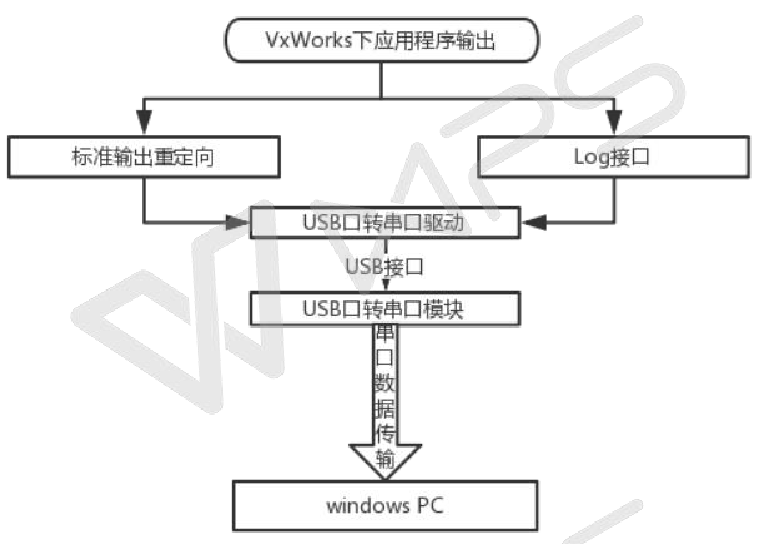
\includegraphics[width=.9\textwidth]{./graphics/debug-system-diagram.pdf}
\caption{调试通道整体结构图}\label{fig:debug-system-diagram}
\end{figure}
	
	整个调试通道主要分为两个模块:应用层的接口模块、USB口转串口模块。
	
	提供给应用层的接口模块负责将系统应用层的输出通过我们的USB口转串口驱动程序传输到windows PC机,输出的形式包括特定内容的格式化的输出和普通的重定向的输出,格式化的输出我们会使用自定义的Log接口进行格式控制,为此我们设计了一个自定义的Log协议格式,其中的内容包含有调试级别、调试信息所在的文件、调试信息所处的行号、输出该条调试信息的时间等;重定向的输出包括RTP模式下的重定向和task模式下的重定向,VxWorks中对于这两种模式需要使用不同的重定向方式。
	
	USB口转串口模块用于在VxWorks上实现一个USB口转串口驱动程序,负责将上层应用的信息传输到windows PC,包括一个特定需求的驱动程序的实现和一个普通的驱动程序的实现。特殊需求的驱动程序相对于普通的驱动程序而言在流程和结构上进行了修改,以使其达到特定的要求,具体的实现我们会在第三节进行介绍。两种实现方式中都会包含有驱动程序加载、卸载模块,设备的打开、关闭、读、写、控制模块。同时在驱动程序中还需要一个数据的管理模块,我们会使用循环缓冲区来管理数据。


\section{关键技术}

\subsection{VxWorks驱动开发}
	
	在VxWorks当中使用I/O子系统来管理设备驱动,I/O 子系统在整个VxWorks当中起着承上启下的作用,各种类型的设备都必须要向I/O子系统进行注册才能够被内核访问,I/O子系统在VxWorks当中的作用是维护系统设备表、系统驱动表、系统文件描述符表\cite{VxWorks内核解读}\cite{曹桂平2011VxWorks}。设备驱动在VxWorks中就靠这三个数据结构来进行管理,所以对于设备驱动而言非常重要。设备驱动程序初始化时会对硬件完成初始化的配置,同时会向I/O子系统注册自己,注册之后I/O子系统才能找到该驱动。

\subsubsection{VxWorks I/O 系统}
	通常操作系统为了应用程序的平台无关性都会为应用程序提供一套标准的接口,VxWorks也不例外,它为应用层的提供了接口函数有creat()、open()、unlink()、remove()、close()、rename()、read()、write()、ioctl()、lseek()、readv()、writev()等\cite{陈洋2007VxWorks}\cite{Wu2008Implementation}\cite{Zhang2010Design},我们通常将其称作为标准I/O 库函数。
	使用库函数可以在对应用层的程序进行开发和移植的时候使用同一套接口,这给应用程序的编程人员带来很大的方便,大大提高了其开发效率,避免了重复工作,而对于操作系统而言它需要通过调整底层驱动或者操作系统中间层来为标准I/O接口的实现提供支持。
	
	在Mac OS、Linux、或Windows当中会把这套接口以标准库的形式呈现,但是在VxWorks中它们是由系统的内核实现的,直接以内核文件的形式提供的,它们都位于ioLib.c文件下\cite{VxWorks内核解读}。之所以是以内核文件的形式来提供,是因为VxWorks当中不会区分用户态和内核态,这是VxWorks与通用操作系统的一个很大的不同点。在Vxworks当中所有的内核函数都可以不加限制的由用户程序直接进行调用,这样就减少了中断转入内核态再继续执行这一个过程,这对于强实时性系统而言极为重要,因为这样减少了时间开销,但是这样实现的一个缺点是减少了系统使用权限上的限制,为内核带来了很大的不安全性,极易导致内核的崩溃,所以VxWorks系统上应用程序的开发和使用对开发人员的要求比较高。
		
	VxWorks中I/O调用结构如\autoref{fig:I/O调用}所示。
	\begin{figure}[!h]
\centering
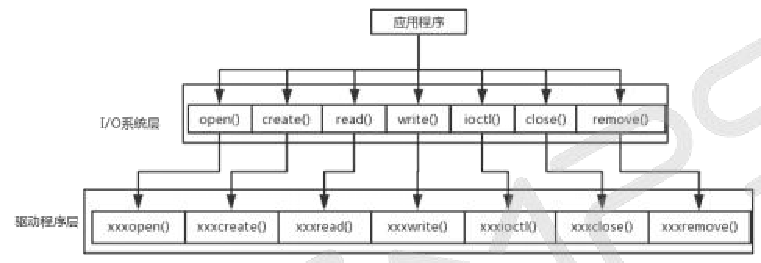
\includegraphics[width=1.0\textwidth]{./graphics/IOCall.pdf}
\caption{I/O调用}\label{fig:I/O调用}
\end{figure}

	
\subsubsection{系统设备表}
	系统设备表是VxWorks中为了管理系统上的所有设备而使用的一个链表,系统设备表中每一个节点都是一个DEV\_ HDR类型的结构体,系统会将每个设备DEV\_ HDR连接在如\autoref{fig:VxWorks系统设备示意图}所示的系统设备表中。DEV\_ HDR是wind内核规定的每一个设备都必须要具有的一个数据结构,且必须是设备自定义结构的第一个成员,之后系统只会使用这个结构来代表该设备。DEV\_ HDR结构体当中只包含有三个成员:一个设备链表节点;一个设备驱动号;一个指向设备名的指针。
	其定义如\autoref{fig:DEVHDR} 所示。

\begin{figure}[!h]
\centering
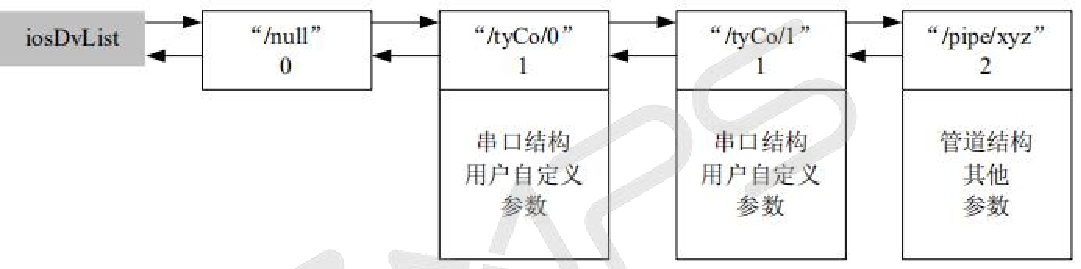
\includegraphics[width=1.0\textwidth]{./graphics/vxworks-device-link.pdf}
\caption{VxWorks系统设备示意图}\label{fig:VxWorks系统设备示意图}
\end{figure}
	
\begin{figure}[!h]
\centering
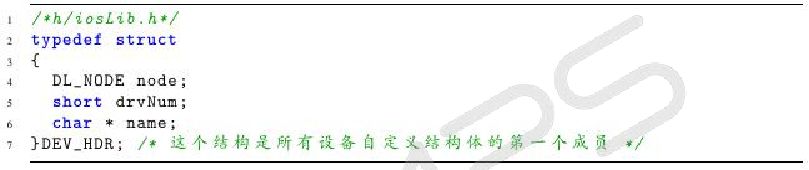
\includegraphics[width=1.0\textwidth]{./graphics/DEVHDR.pdf}
\caption{DEV\_ HDR结构体}\label{fig:DEVHDR}
\end{figure}

同时VxWorks系统提供了一个设备的注册函数iosDevAdd( DEV\_ HDR *pDevHdr, char *name, int drvnum),该函数用来将一个设备添加到系统设备表当中,系统设备表在每次添加设备时就会在表中增加一个节点表示该设备,删除设备时就会将该设备的节点从表中删除,一个设备添加到系统之后,就可以使用open()函数对其进行操作,open()会通过将传递过来的设备名与系统设备表当中进行设备名匹配来完成设备的打开操作,匹配的原则是最佳匹配,匹配成功之后就可以实现文件与设备的连接\cite{刘小军2008基于},之后就可以使用相对应的注册的设备驱动进行其他的文件操作。

\subsubsection{系统驱动表}	
	系统驱动表用于管理当前注册到I/O子系统下的所有驱动程序,既可以是直接驱动硬件工作的驱动程序,也可以是注册到I/O子系统下的驱动中间层\cite{VxWorks内核解读}。
	在VxWorks中系统驱动表的底层实现是一个数组,数组中的每一个元素就是一个系统驱动表的表项,每一个表项都是一个 DRV\_ ENTRY 类型的结构体,该结构定义在内核的头文件iosLibP.h当中,其定义如\autoref{fig:DEVENTRY}所示。
	
\begin{figure}[!h]
\centering
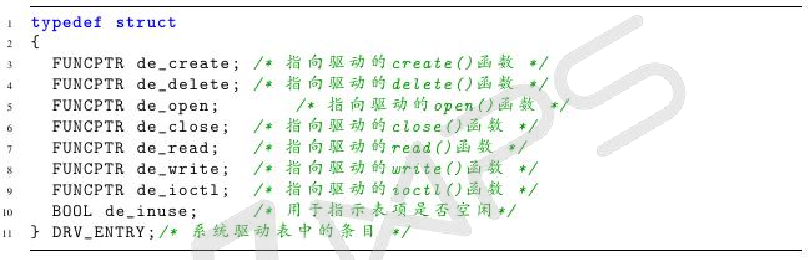
\includegraphics[width=1.0\textwidth]{./graphics/DEVENTRY.pdf}
\caption{DEV\_ ENTRY结构体}\label{fig:DEVENTRY}
\end{figure}

	DEV\_ ENTRY结构体当中的大多数成员都是函数指针,他们用于指向所注册的驱动程序中的一个用于完成特定功能的实际函数,这些函数的功能要符合IO系统预定义好的规则,这些函数被加入到系统驱动表中之后就可以完成与用户层提供的标准函数接口对接\cite{VxWorks内核解读}\cite{VxWorksDriverAPI}\cite{Wind2003VxWorks}。在DEV\_ ENTRY结构体当中唯一不是函数指针的成员是一个布尔类型的 de\_ inuse 成员,若该成员为FALSE则表示该表项目前是未被使用的状态,即该表项没有被任何的驱动所注册。

	VxWorks当中给我们提供了一个驱动的注册函数iosDrvInstall(),使用该函数注册我们的驱动之后,系统驱动表就会分配一个未被使用的表项给该驱动,然后使用iosDrvInstall()所提供的的参数来填充系统驱动表当中的指针,并将de\_ inuse置为TRUE的状态,一个驱动程序不需要实现所有的IO函数,对于实现的函数,在注册时直接将其指针置为NULL即可。


\subsubsection{系统文件描述符表}
	系统描述符表用于管理当前系统中所打开的所有文件描述符,VxWorks中系统描述符表的底层实现也是一个数组。每次执行open()调用成功之后,系统就需要从系统描述符表中分配一个表项给程序使用,并将文件描述符的表项索引作为文件描述符的ID返回给应用程序。之后应用程序直接通过这个ID就可以对文件进行操控,无需每次都是用文件名。
	在VxWorks中,标准输入、标准输出、标准错误输出虽然使用 0,1,2 三个文件描述符来表示,但是它在底层的实现上可能并不是占用了三个文件描述符表的表项,而是只占用一个表项,即三个文件描述符指向同一个文件描述符的表项\cite{VxWorks内核解读}\cite{An2003Implementation},这一点是需要注意的。
		
	
系统文件描述符表中每一个表项都使用 FD\_ ENTRY 这个结构体来表示,这个结构定义在内核的头文件iosLibP.h 中,其定义如\autoref{fig:FDENTRY}所示。


\begin{figure}[!h]
\centering
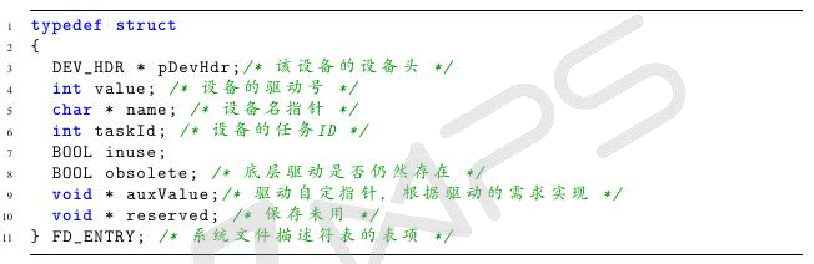
\includegraphics[width=1.0\textwidth]{./graphics/FDENTRY.pdf}
\caption{FD\_ ENTRY结构体}\label{fig:FDENTRY}
\end{figure}


用户的应用程序每次使用open()系统调用系统文件描述符表中就会增加一个有效表项,该表项的FD\_ ENTRY结构体会根据open()调用的内容来进行填充,每一个文件能够进行的open()调用是有限制的,因为数组的容量是固定的,每个驱动的FD\_ ENTRY结构数组满了之后就无法再对这个设备进行open()操作,此时 open()函数将会失败返回\cite{VxWorks内核解读}。系统会在表中的索引偏移 3 (0、1、2被系统占用)之后找一个最先找到的未使用的id作为文件描述符返回给用户。
	
\subsection{VxWorks 中的通信机制}
	
	任务间的通信机制用于协调多个任务之间的活动,在我们的USB口转串口驱动程序当中需要使用任务间的通信机制来确保对驱动内部缓冲区中的数据正确、有序的读写,VxWorks内核当中为我们提供了丰富的任务间通信机制,包括共享内存、信号量、消息队列、管道、信号、Sockets等。我们主要介绍一下VxWorks任务中使用较多的信号量、消息队列和管道这三种机制,它们在本质上都是使用的共享物理内存机制,只是这块共享的内存不是由用户进行管理,而是交由内核进行管理的,这种实现机制可以使任务间通信安全有序的进行\cite{胡明民2012基于实时操作系统}\cite{冯云贺2014基于}。

\\

\noindent \textbf{1. 信号量}
	
	信号量是一种在程序的设计当中最常使用的通信机制,其主要作用是线程间的同步和互斥。VxWorks中提供POSIX信号量的同时还设计了专门的wind信号量,POSIX信号量的使用主要是为了方便程序的移植。
	和POSIX信号量的不同之处在于,VxWorks中设计的wind信号量为VxWorks系统进行了高度的优化,使得其更适用于实时操作系统,能够更快的实现任务间通信。VxWorks中信号量是一个指向SEMAPHORE类型的结构指针,提供了二进制信号量、互斥信号量、计数信号量三种类型的信号量机制,他们适用于解决不同类型的问题。
	
\begin{itemize}
\item 二进制信号量\\
	二进制信号量是最快、最通用的信号量,既可以用于同步也可以用于资源计数。wind的二进制信号量所需系统开销最少,适用于高性能的需求。二进制信号量在资源可用时标记为FULL,在资源不可用时标记为EMPTY。在VxWorks中二进制信号量使用函数semBCreate()来创建,二进制信号量的提取和释放过程如\autoref{fig:二进制信号量的提取与释放过程} 所示。

\begin{figure}[h]
\centering
  \begin{subfigure}[b]{1.0\textwidth}
  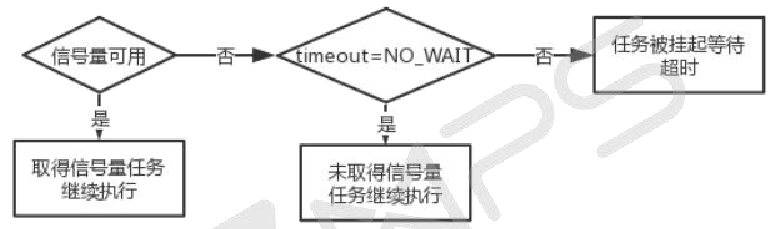
\includegraphics[width=\textwidth]{./graphics/erjinzhiTiQu.pdf}
  \caption{提取信号量}\label{fig:cp2102Front}
  \end{subfigure}
  ~
  \begin{subfigure}[b]{1.0\textwidth}
  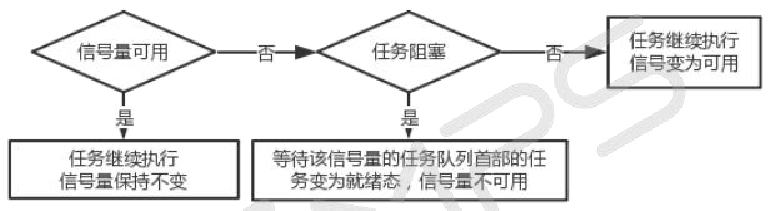
\includegraphics[width=\textwidth]{./graphics/erjinzhiShiFang.pdf}
  \caption{释放信号量}\label{fig:cp2102Rear}
  \end{subfigure}
\caption{二进制信号量的提取与释放过程}\label{fig:二进制信号量的提取与释放过程}
\end{figure} 


\item 互斥信号量\\
	互斥信号量可以看做是一种特殊的二进制信号量(资源数为1),它优化了互斥、优先级继承、删除安全等问题,这使得它能够更好的服务于任务间的互斥需求;互斥信号量的基本行为和二进制信号量是一致的,但是互斥信号量只能够用于互斥,不能够用于同步,该信号量只能够由获得的该信号量的进程来进行释放,不能够由其它的进程进行释放。它使用SEM\_ INVERSION\_ SAFE和SEM\_ Q\_ PRIORITY选项来使得该信号量能继承优先级算法,以此解决优先级的倒置问题;使用SEM\_ DELETE\_ SAFE选项来解决删除安全问题,在VxWorks中互斥信号量使用系统提供的semMCreate()函数来创建;
	
\item 资源计数信号量\\
	资源计数信号量也是一种特殊的二进制信号量(资源数较多),它会跟踪信号量增加、删除的次数,每次释放一个信号量,内部的计数器就会执行加一操作,每次提取一个信号量,内部的计数器就会执行减一操作,当计数器为0时,表示没有可供使用的资源,此时提取信号量的操作就会被阻塞,在VxWorks中资源计数信号量使用系统提供的semCCreate()函数来创建。

\end{itemize}
	
三种信号量的释放操作都是使用semGive()函数;提取操作都是使用semTake()函数,在提取信号量是我们可以选择是否允许超时,超时可以作为解决阻塞的一种方法。

	\\
	
\noindent \textbf{2. 消息队列}

	消息队列是一种在消息传输的过程中保存消息的容器,它给互相合作的任务间提供了一种通信机制。如\autoref{fig:消息队列}是消息队列实现任务间通信的一种方式。
	和信号量类似,VxWorks中也支持POSIX消息队列,其目的主要是为了方便移植和程序的兼容,同时VxWorks中也设计了专门用于Wind的消息队列,位于msgQLib文件当中。VxWorks中提供函数msgQCreate()来创建一个消息队列;msgQDelete()用于删除一个消息队列;msgSend()用于向消息队列中发送一个消息;masgQReveice()用于从消息队列中提取一个消息。
	
	在wind中消息队列是使用结构数组来实现的,在创建消息队列时必须指定一个消息的最大长度和队列中能够容纳的消息数量,这一特性使得其在任务间传递较多信息时存在的很大的局限性\cite{冯云贺2014基于}。
	
\begin{figure}[!h]
\centering
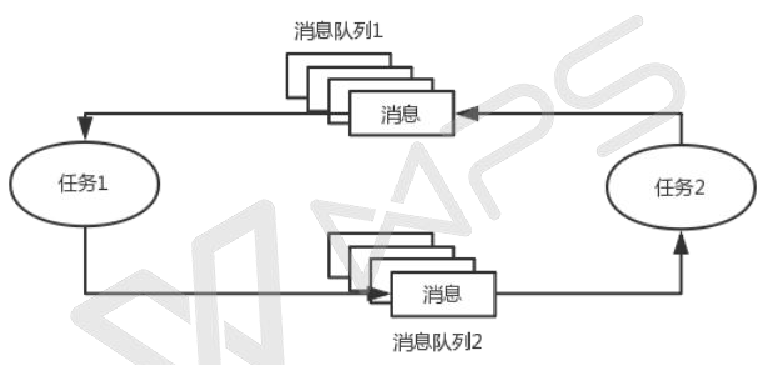
\includegraphics[width=0.9\textwidth]{./graphics/messageQueue.pdf}
\caption{消息队列实现全双工通信}\label{fig:消息队列}
\end{figure}	
				


\\	
	
	\noindent \textbf{3. 管道}
	
	管道也是一种基本的进程间通信机制,包括命名管道和匿名管道。VxWorks内核当中使用环形队列的方式来实现管道,管道提供了比消息队列更流畅的信息传递机制,可以像文件一样进行读写。命名管道具有一个与之关联的路径名,因此任何的进程间都可以用它进行通信,命名管道是双工的数据可以双向流动;非命名管道一般用于父子或兄弟进程间通信,非命名管道是半双工的,数据只能向一个方向流动。

\\
	
\noindent \textbf{4. 任务间特殊的通信机制--信号} 

	信号通常用于通知一个进程发生了异步事件,也被称为软中断。通常收到信号的进程通常可以选择三种方式来处理:一是使用一个信号处理函数处理;二是选择忽略该信号;三是使用系统默认的处理方式处理。
Wind内核同时支持UNIX BSD风格的信号和POSIX 信号,但是Vxworks中的信号处理机制有些特别之处,对于SIGKILL,SIGSTOP这类的信号,在通用操作系统上是不允许用户修改其默认处理函数的,但是在 VxWorks 操作系统中可以对任何信号的处理函数都可以进行更换的。



\subsection{USB技术}
	USB(Universial Serial Bus)作为PC领域的最新型的接口技术,目前已被各个PC厂家所支持,并且在各类外设当中都广泛的采用USB接口。USB的开发技术也已经很成熟,通用串行总线开发者论坛(USB Implementers Forum,USB IF)目前制定了三种USB接口标准:USB1.1,USB2.0和USB3.0。USB采用菊花链的形式连接所有的设备,最多可以连接127个设备,USB的总线拓扑结构如\autoref{fig:USB体系结构}所示
\begin{figure}[!h]
\centering
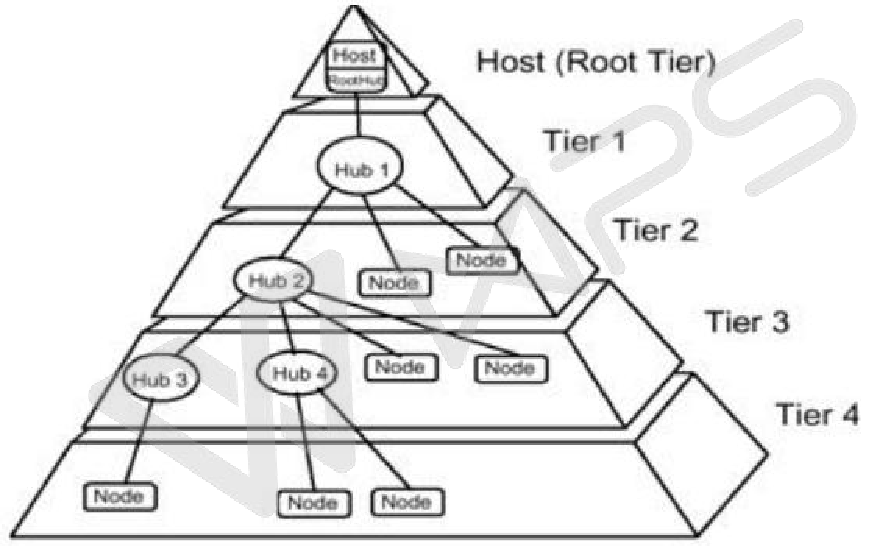
\includegraphics[width=1.0\textwidth]{./graphics/usb-structure.pdf}
\caption{USB总线拓扑结构}\label{fig:USB体系结构}
\end{figure}


USB的体系结构由三个部分组成,分别是USB主机(Host)、USB集线器(Hub)、USB设备(Device)。其中我们需要了解的关键部分是USB主机和USB设备。

\\
	
\noindent \textbf{1. USB主机}
	
	USB主机是USB体系中的核心,且系统中只允许一个USB主机存在。USB主机上的USB接口是USB主控制器,其控制着总线上所有USB设备数据通信。对于USB的体系结构而言,其数据的传输都是USB主机端发起的,非主机端(设备端)只能够被动的进行响应。USB主机需要完成的功能包括检测设备的热插拔、管理主机和设备之间的信息(控制和数据)流\cite{李雪红2004USB}\cite{莫宏伟2001USB}。


\\

\noindent \textbf{2. USB设备}

	USB设备指的是提供具体功能的而外部USB设备,是相对USB主机而言的,它们受USB主机的控制,只能对主机的请求进行被动响应。USB主机端会在检测到USB设备的动作之后会通过默认管道和USB设备进行通信,对其进行必要的初始化配置,并给设备提供适合的驱动程序(如果有的话),一个USB设备会通常会有很多的属性,它会通过这些属性来完成主机的配置要求。一些USB设备的属性如下:
	\begin{itemize}
	\item \textbf{描述符(Descriptor)属性}\\
	描述符是USB协议中定义的一套用来描述USB设备的功能和属性的固定结构,我们可以通过描述符了解设备的各种属性,描述符又分为设备描述符、配置描述符、接口描述符、端点描述符、字符串描述符\cite{张杰2008基于}\cite{边海龙2004USB}除此之外,设备还可以提供自己专用的描述符,分为设备类描述符和供应商自定义描述符,我们使用的USB口转串口设备就不属于一个标准的USB设备,它会为我们提供供应商自定义的描述符,我们使用需要使用它来对设备进行识别。
	
	\item \textbf{类(Class)属性}\\
	由于USB协议支持许多的外围设备,而这些设备又可以根据功能来分成一些相近的类,如打印机类、键盘类等。这样主机端就可以为这些功能相近的设备提供一个类驱动,类驱动可以用于驱动所有属于同一类的设备,不需要再为每一个设备提供一个完整的驱动程序。这大大的方便的设备的制造商,他们的设备只需要符合某一类的驱动,就可以使用该类驱动程序来驱动其设备,之后只需要实现简单的包含有设备特性的客户端驱动即可,若设备没有特殊的特性,则直接使用类驱动即可\cite{李雪红2004USB}。	
	
	\item \textbf{功能(Function)/接口(Interface)属性}\\
	功能或接口是USB协议中定义的设备的某种能力,Function是从功能角度来说的,从设备的角度来说,被称为Interface。对于一个设备他可以拥有很多个不同的接口,每一个接口负责完成设备的一个特定的功能,并且这个接口具体实现什么样的功能并不是固定的,当USB设备处于可配置状态的时候能够通过控制命令来改变某一个接口的功能,一个接口能够具有什么样的功能会在USB的接口描述符中进行描述。
	
	\item \textbf{端点(Endpoint)属性}\\
	端点是USB设备与USB主机逻辑上的通信流的终点,每个设备都拥有一个可独立进行操作的端点集合,且每个端点在使用时都要先初始化其数据传输方向(IN/OUT),即使端点号相同但是传输方向不同的通信点也是不同的端点\cite{李雪红2004USB}。
	
	\item \textbf{管道}\\
	管道可以看做是设备上的一个端点和主机上的软件的联合体,设备和主机间的数据传输要基于管道进行。在USB的通信过程中首先要建立一个管道才能够进行数据的传输,USB设备在和主机通信时都会建立一个默认的管道,这个管道对应的端点是默认端点0,之后需要自己使用其它的端点来建立我们的数据传输过程中需要使用的输入或输出管道。在我们的USB口转串口驱动中会为每一个设备建立两个管道,一个批量输出管道和一个批量输入管道。
	
	\item \textbf{设备地址}\\
	设备地址用于区分USB系统中的一个USB设备的特殊标识,设备地址会在设备初始化之后由主机进行分配且是唯一的。设备地址单元共有7bit,其中地址0是缺省地址,在设备初始化的时候使用,理论上系统可以区分127个USB设备\cite{李雪红2004USB}。
	\end{itemize}	



\noindent USB规范规定了USB主从设备之间的四种传输方式,每种方式有各自的用途\cite{USB总线接口开发指南}:

\begin{itemize}
\item \hei{控制传输}:控制传输USB传输方式中最重要、最复杂的一种,它适用于少量、对时间和速率无要求的场合,一个USB设备插入主机之后就是使用这种传输方式来读取设备的地址和描述符等信息。所有的设备都会在其0号端点的缺省管道当中支持控制传输\cite{张杰2008基于}。
\item \hei{批量传输}:批量传输有两种最基本的事物类型:BULK\_ IN和BULK\_ OUT,其主要用于处理对数据传输速率不是很高的情况,批量传输使我们的USB口转串口设备所使用的主要传输传输方式,每次有数据需要传输时我们都会构建一个IRP使用批量传输将其传出或传入。
\item \hei{中断传输}:中断传输也有两种基本的事务:IN和OUT,其主要是为那些要快速实现主机和设备的交互,但是数据量很小、对服务时间有要求的情况而准备的。
\item \hei{等时传输}:等时传输也是由基本的IN和OUT两种事务组成,主要用于处理大量、恒速、对时间周期有要求的数据。等时传输只有全速和高速设备才支持,低速设备不支持\cite{张杰2008基于}。
\end{itemize}


	

\section{本章小结}
	本章重点介绍了本次的VxWorks调试通道的整体架构,并介绍了介绍了各个部分的设计方案,最后介绍了在本次的设计当中所需要使用关键技术和所需了解的重要知识,主要包括VxWorks下的驱动开发必须的结构、驱动中所需使用的VxWorks的通信机制、缓冲区技术、USB技术。下面将要讨论VxWorks下的调试通道的详细的设计细节和具体的实际机制。



























\clearpage

% 本章的介绍性内容过多,将前两章合成一章即可,内容将其删减,前面几张的内容过多,从实现部分开始应该从24页左右开始。

\chapter{驱动程序的设计和实现}
	在此我们需要编写一个VxWorks下的USB口转串口的驱动程序,在编写驱动程序之前我们有必要先了解一下VxWorks下驱动的软件结构,USB口转串口的流程以及相关的工作原理。
\section{VxWorks设备驱动概述}
	驱动程序简单来说就是用来某个硬件的配置,使其能够完成固有功能的程序。驱动程序直接与硬件设备交互,其大多数的工作就是操作硬件相关寄存器。设备中的寄存器在系统掉电之后其内容会丢失,系统上电复位时其会复位到一个默认值,通常默认状态下的硬件是不能正常工作的,如中断使能被屏蔽,工作使能位也被屏蔽,还有一些决定硬件工作情况的关键控制寄存器也需要被重新配置。而这些工作都有赖于设备驱动完成。驱动一般都作为操作系统内核组成的一部分,即便现在很多系统支持驱动的动态加载,但是驱动代码在执行时,依然是以内核代码模式进行执行的,换句话说,驱动代码具有系统特权级,除了其自身资源,对应硬件设备资源,其还对操作系统资源具有完全的访问权。所以一个驱动程序如果存在 BUG,将直接会导致整个操作系统的崩溃。故调试驱动是一项十分关键的工作,必须对驱动进行仔细检查,并需要经受长时间运行考验。底层驱动的调试过程是同时对硬件和驱动进行验证的过程。底层驱动很多时候用来定位硬件设计错误或者硬件芯片本身可能的问题,故底层驱动程序员必须对所要驱动的硬件设备有一个比较充分的了解,以及对与硬件交互的其他硬件或外界环境也需要有一个比较清楚的理解。
	
	在VxWorks中驱动程序对上需要匹配操作系统提供的一套规范接口,对下必须驱动硬件设备进行工作,其起着一个关键的中间转换角色,将操作系统的具体请求转换为对硬件的某种操作,让所有的硬件对操作系统的一套内部规范接口进行响应,屏蔽了硬件的所有复杂性,应用层对于某个设备的操作通过操作系统提供的一套标准接口完成,操作系统最终将这些操作请求传递给驱动程序,驱动硬件完成这些请求。	
	
	在VxWorks系统中,在控制器权转到设备驱动程序之前,用户的请求进行尽可能少的处理。VxWorks I/O系统的角色更像是一个转接开关,负责将用户请求转接到合适的驱动例程上。每一个驱动都能够处理原始的用户请求,到最合适它的设备上。另外,驱动程序开发者也可以利用高级别的库例程来实现基于字符设备或者块设备的标准协议。因此,VxWorks的I/O系统具有两方面的优点:一方面使用尽可能少的使用驱动相关代码就可以为绝大多数设备写成标准的驱动程序,另一方面驱动程序开发者可以在合适的地方使用非标准的程序自主的处理用户请求。

\subsection{设备驱动的功能以及分类}\label{sec:设备分类}
	
	驱动程序是位于用户和硬件之间一个软件层,驱动程序员有完全的决定权决定一个硬件设备以何种形式呈现给用户,不同的驱动程序可以使得同一个硬件设备以不同的方式对用户可见。我们可以将一个实际块设备以字符设备对用户可见,将一个实际Flash设备以硬盘设备对用户可见,以何种形式表现一个实际设备完全由底层驱动控制。驱动程序员可以提供一系列方式让用户对设备进行控制,甚至可以让用户直接操作硬件设备的每一个寄存器,由用户在寄存器层次对硬件设备进行操作;或者只提供一个读或写操作,屏蔽其他所有操作等等。
	
	故从宏观角度而言,驱动程序实现的功能即提供一种底层服务机制供用户进行选择。从微观角度而言,驱动程序需要对下配置硬件寄存器,完成对设备数据的读写,对设备本身的控制,对上使得设备能够响应用户的服务请求,这些服务请求如下:打开设备;读写设备;控制设备;关闭设备。

驱动一般具有如下的五个基本功能:
	\begin{enumerate}
	\item 完成与设备有关的设备寄存器的初始化。其目的是为了使硬件平台工作在确定的状态下。
	
	\item 完成设备的打开。该功能在本质上是检查用户指定要访问的设备是否存在。
	
	\item 完成设备的关闭。其作用是释放设备在使用时占用的系统资源。
	
	\item 设备与系统数据通信。其本质就是完成的对设备的读写过程。也是驱动程序所需要完成的主要的功能。
	
	\item 对设备的控制操作。 在使用设备的过程中,需要根据实际的需求来设置设备的工作状态。
	\end{enumerate}	
	
基于以上设备所需要实现的五大基本功能,我们可以得出凡是基于VxWorks内核调用的驱动程序不外乎以下的组成部分:

\begin{enumerate}
\item 设备驱动函数的注册函数。驱动开发人员必须要开发响应的函数将驱动程序的功能注册到设备驱动程序列表中,以便挂接到I/O系统。

\item 设备驱动的卸载函数。若系统不再使用设备,需要将其卸载掉,以节约系统资源

\item 设备的打开和关闭函数。这两个函数是相伴的,有打开操作就必须有关闭操作。

\item 设备的读写函数。主要完成设备的外设和CPU之间的数据交换。

\item 设备的控制函数。在使用设备的过程中,需要对设备的工作状态进行控制。

\item 中断服务函数(ISR)。响应外设的中断请求。
\end{enumerate}\\
根据设备的工作方式和数据的存储或者来源不同,可以将设备分为三大类:
\begin{itemize}
\item \hei{字符设备类型}

	字符设备即以字节流的方式被访问,就如同一个文件,但不同于文件之处是字符设备一般不可以移动文件偏移指针,而只能顺序的访问数据。终端设备以及串口设备都属于字符设备类型。字符设备驱动至少需要实现 open,close,read 和 write 四个系统调用底层实现函数。

\item \hei{块设备类型}

	块设备一般通过文件系统访问。而块设备的最多使用方式也是文件方式。块设备一般不能对单个字节进行访问,而是一个块的方式(如硬盘以一个扇区(512B)为单元进行访问)进行。块设备允许同一数据的反复读取和写入。最典型的块设备就是硬盘,Flash 设备也是一种块设备。
	
\item \hei{网络设备类型}

	用于与网络上其他主机进行通信。其数据读取方式有些类似于字符设备,不可以对同一数据进行反复读写,只能顺序读写数据。且该类型设备区别于字符设备和块设备的一个很大的不同是,其不提供文件节点,任务要访问一个网络设备必须使用另一套网络套接字接口函数进行,与文件系统则完全不相关。网络设备底层数据传输上以块的方式进行,但是又不同于块设备中数据块的概念,网络设备中块的大小可以改变,但是有一个区间范围。
	
\end{itemize}

	以上只是设备类型的划分方式之一,事实上,按以上的划分标准,某些设备接口在某些情况下可以表现为任意以上三种形式之一,如 USB 接口,可以是一个字符设备,如 USB 串口;也可以是一个块设备,如 USB 内存卡;也可以是一个网络设备,如 USB 网络接口。

\subsection{VxWorks设备驱动层次结构}
	
	VxWorks 的I/O框架由ioLib.c 文件提供,但ioLib.c文件提供的函数仅仅是一个最上层的接口,并不能完成具体的用户请求,而是将请求进一步向其他内核模块进行传递,位于ioLib.c模块之下的模块就是iosLib.c。我们将ioLib.c 文件称为上层接口子系统,将iosLib.c文件称为I/O 子系统,注意二者的区别。上层接口子系统直接对用户层可见,而I/O 子系统则一般不可见(当然用户也可以直接调用iosLib.c 中定义的函数,但一般需要做更多的封装,且违背了内核提供的服务层次),其作为上层接口子系统与下层驱动系统的中间层而存在。VxWorks的内核驱动层次结构如\autoref{fig:VxWorks内核驱动层次结构}所示。

\begin{figure}[!h]
\centering
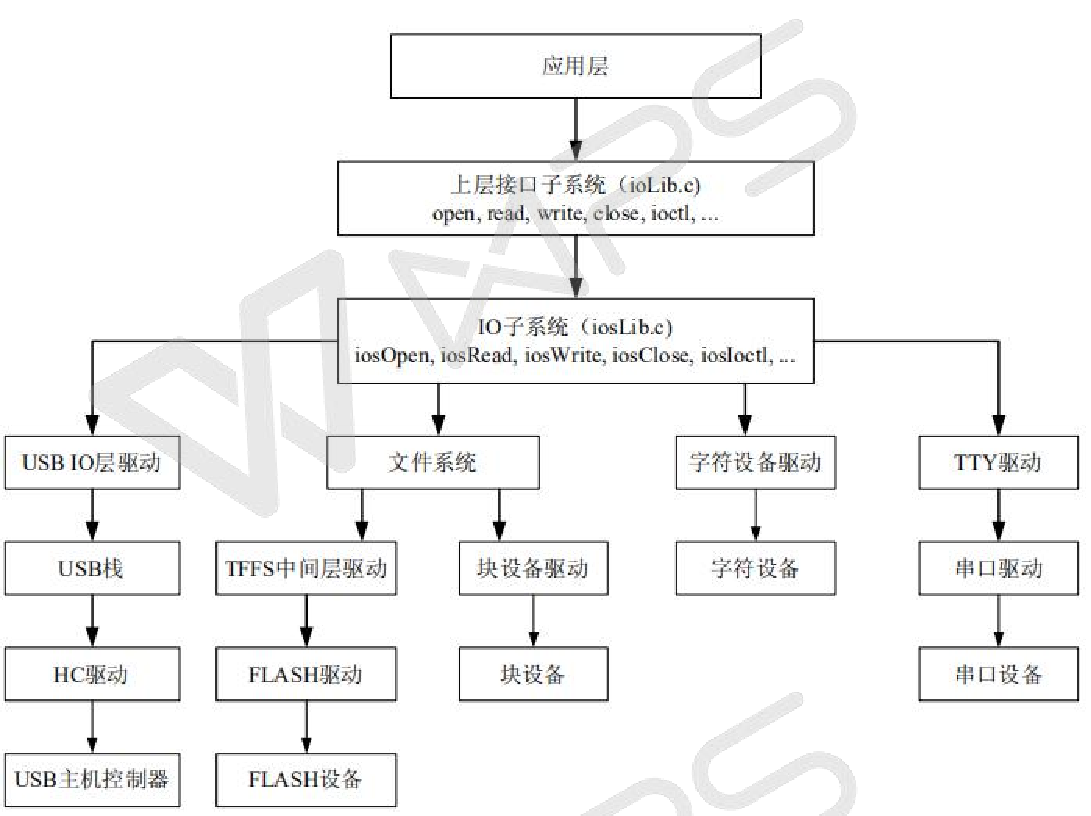
\includegraphics[width=1.0\textwidth]{./graphics/vxworks-kernel-diagram.pdf}
\caption{VxWorks驱动内核层次结构}\label{fig:VxWorks内核驱动层次结构}
\end{figure}
	
	I/O 子系统在整个驱动层次中起着十分重要的作用,其对下管理着各种类型的设备驱动。换句话说,各种类型(包括网络设备)的设备都必须向I/O 子系统进行注册方可被内核访问。所以在I/O 子系统这一层次,内核维护着三个十分关键的数组用以对设备所属驱动、设备本身以及当前系统文件句柄进行管理。需要指出的是,VxWorks文件系统在内核驱动层次中实际上是作为块设备驱动层次中的一个中间层而存在的,其向I/O 子系统进行注册,而将底层块设备驱动置于自身的管理之下以提高数据访问的效率。在这些文件系统中,dosFs 和rawFs 是最常用的两种文件系统类型,在VxWorks早期版本就包含对这两种文件系统的支持。
	
\section{内核驱动的相关结构}
\subsection{系统设备表}
	
	在VxWorks中对于每一个设备都会使用DEV\_ HDR的结构来表示这个设备,DEV\_ HDR的定义如下:
\lstset{language=C}
\begin{lstlisting}
/*h/iosLib.h*/
typedef struct /*DEV_HDR - device header for all device structures*/ 
{ 
  DL_NODE node; /* device linked list node */ 
  short drvNum; /* driver number for this device */ 
  char * name;/* device name */ 
}DEV_HDR;  
\end{lstlisting}

	在该结构中给出了链接指针node(用以将该结构串入队列中),驱动索引号drvNum,设备节点名name。内核提供这个结构较为简单,只存储了一些设备关键部分。底层驱动对其驱动的设备都有一个自定义数据结构表示,其中包含了被驱动设备寄存器基地址,中断号,可能的数据缓冲区,保存内核回调函数的指针,以及一些标志位。最为关键的一点是 DEV\_ HDR 内核结构必须是这个自定义数据结构的第一个成员变量,因为这个用户自定义结构最后需要添加到系统设备队列中,故必须能够在用户自定义结构与 DEV\_ HDR 结构之间进行转换,而将 DEV\_ HDR 结构设置为用户自定义结构的第一个成员变量就可以达到这个目的。
	
	
	驱动程序必须先将设备注册到 IO 子系统中,这个过程也被称为创建设备节点。IO子系统提供了一个简单的被驱动程序调用的设备注册函数iosDevAdd(),该函数原型如下:
\lstset{language=C}
\begin{lstlisting}
STATUS iosDevAdd 
( 
  DEV_HDR *pDevHdr, /* pointer to device's structure */ 
  char *name, /* name of device */ 
  int drvnum /* no. of servicing driver,returned by iosDrvInstall()*/
 ); 
\end{lstlisting}\\
iosDevAdd 函数将一个设备添加到由 IO 子系统维护的系统设备列表中,该列表是一个双向链表,成员通过指针链接在一起,这是由 DEV\_ HDR 结构中 node 成员变量完成的,每当添加设备时,系统都会像链表添加新的节点。系统设备列表由 iosDvList 内核变量指向,系统设备表在系统中的连接方式如\autoref{fig:VxWorks系统设备示意图}所示。系统设备表为open()、close()、remove()这三个函数提供文件与设备的连接,当应用程序执行这三个函数中的一个时,IO系统会将文件名和设备链表中的进行匹配,匹配成功之后就使用这个设备驱动进行文件的其他操作。

\begin{figure}[!h]
\centering
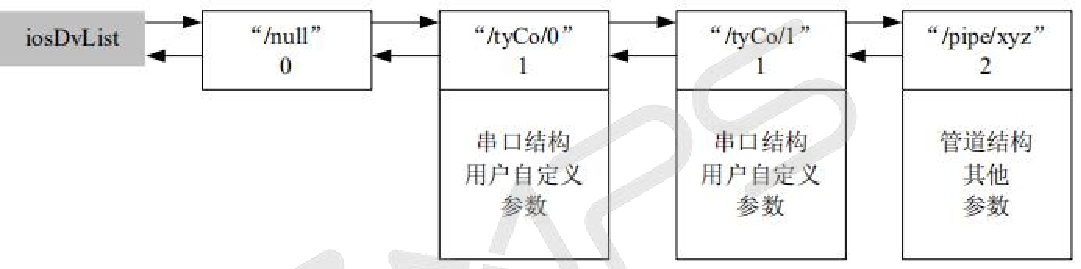
\includegraphics[width=1.0\textwidth]{./graphics/vxworks-device-link.pdf}
\caption{VxWorks系统设备示意图}\label{fig:VxWorks系统设备示意图}
\end{figure}

用户可以在命令行下使用iosDevShow或者是devs来显示系统设备的所有设备,在我们本次所使用的环境中,存在的设备如\autoref{fig:iosDevShow}所示。
\begin{figure}[!h]
\centering
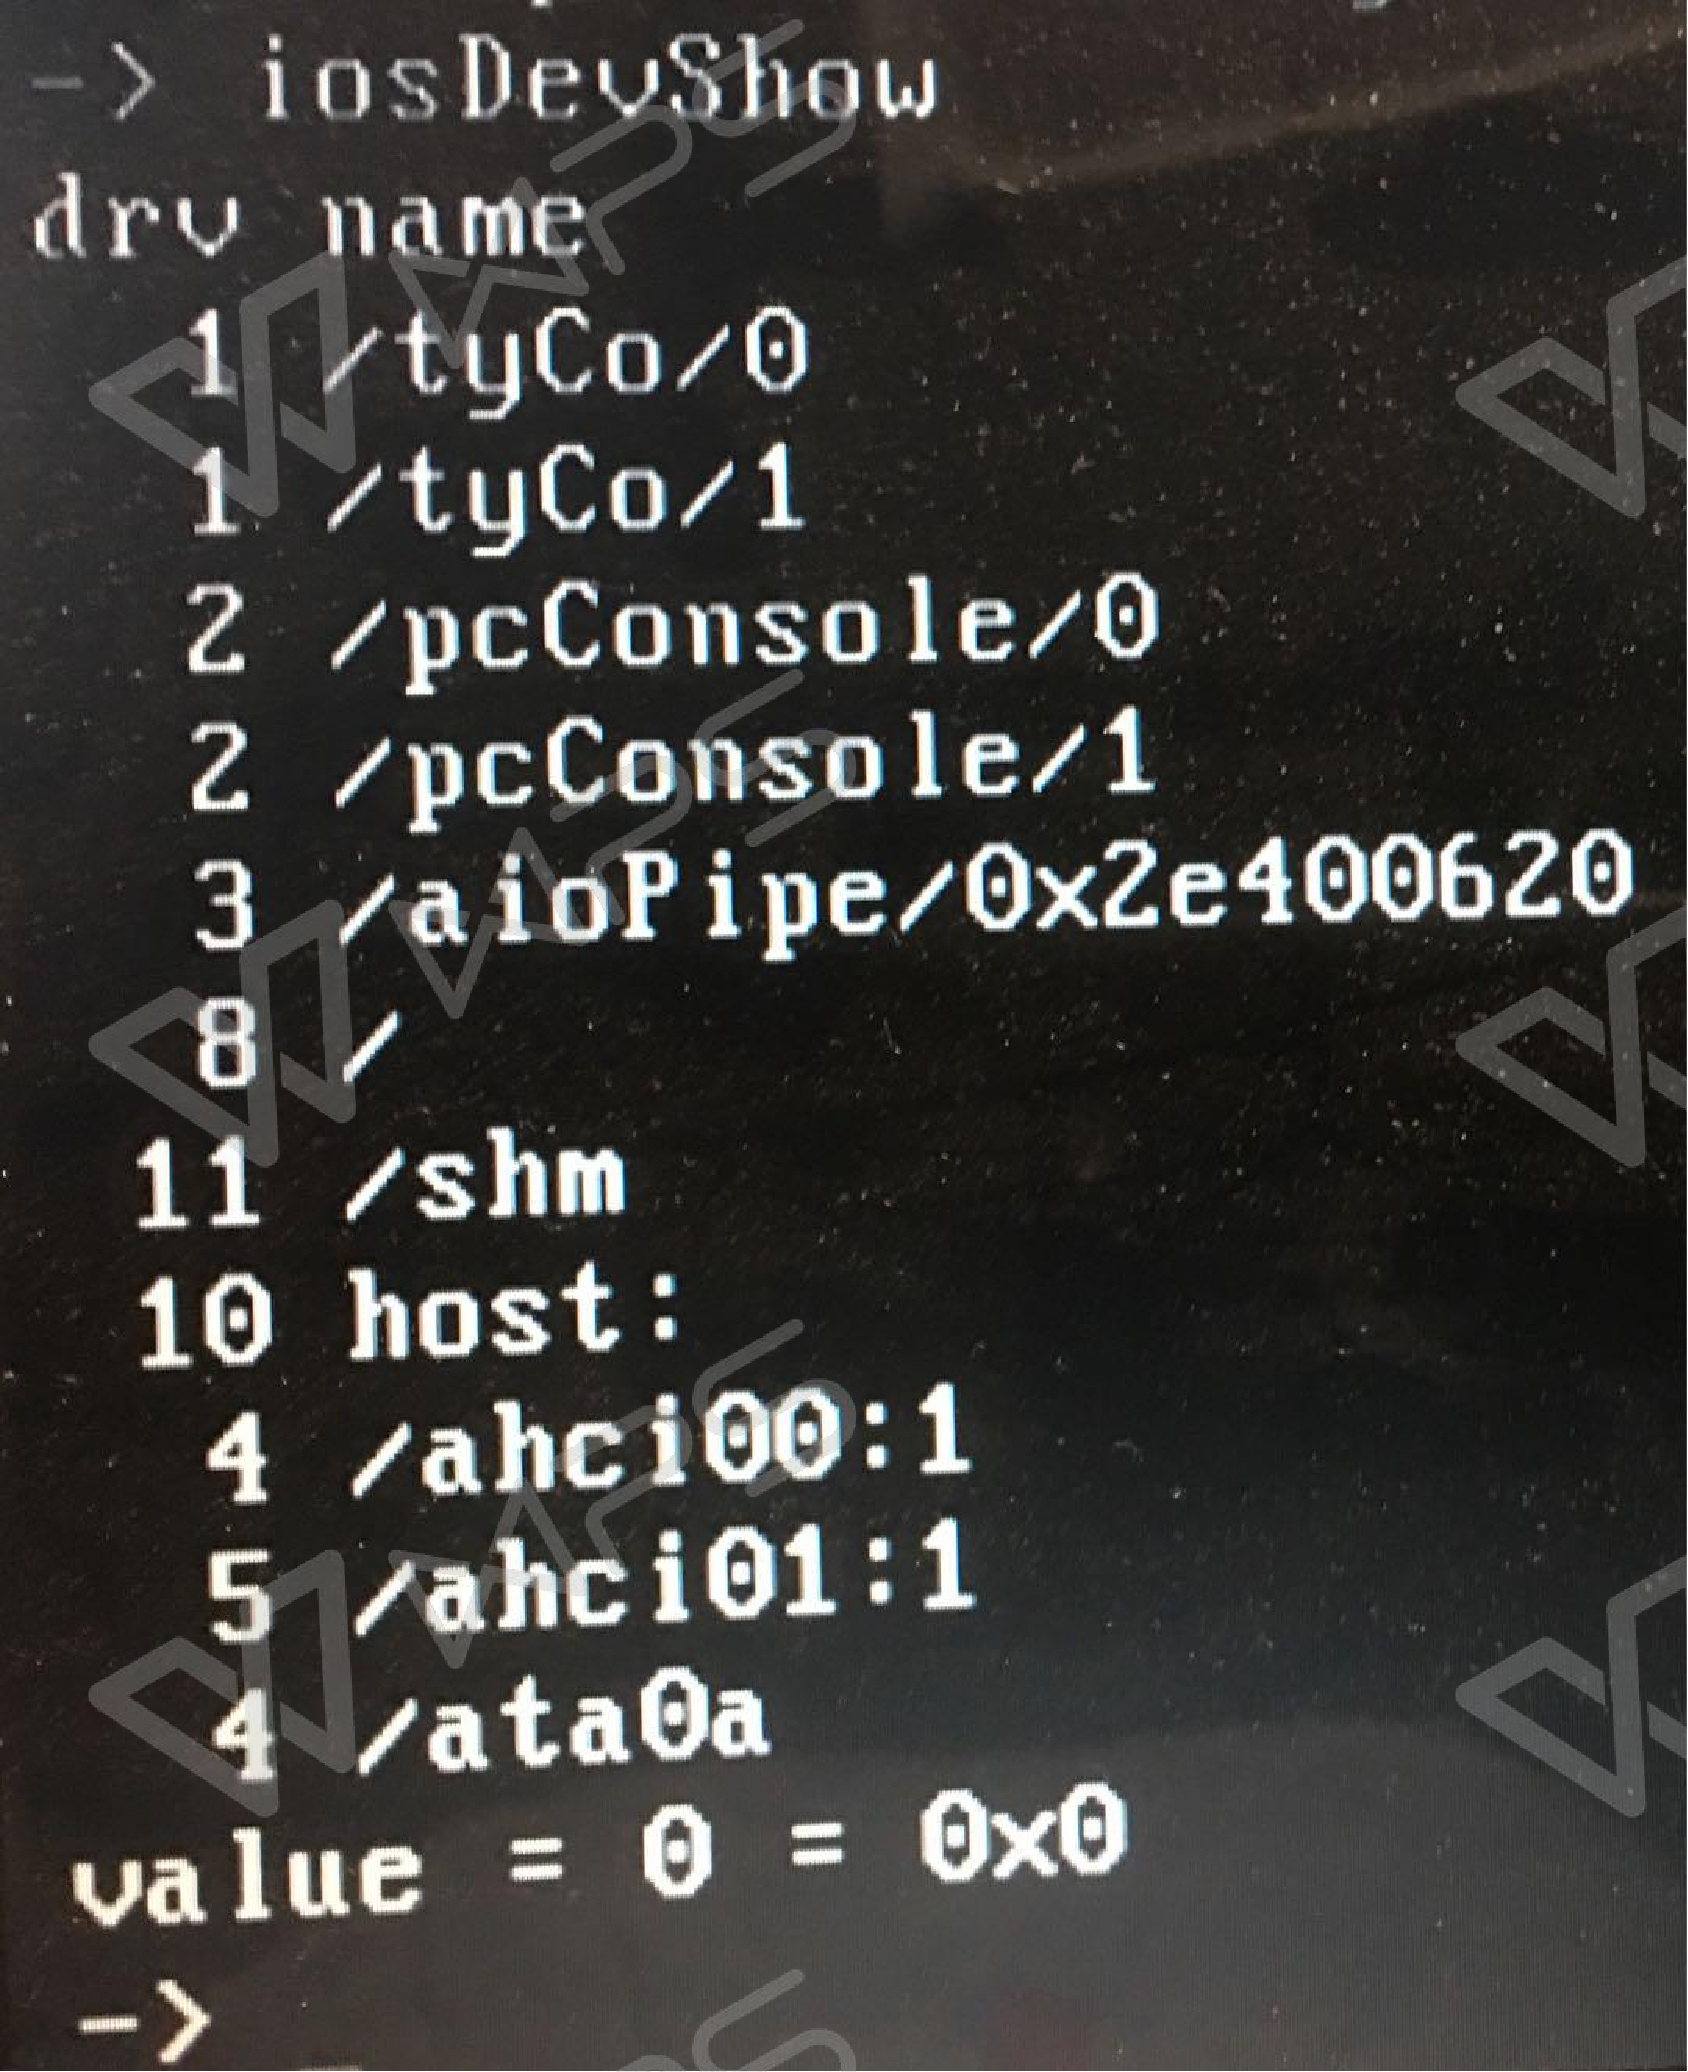
\includegraphics[width=.5\textwidth]{./graphics/iosDevShow.pdf}
\caption{当前系统上的所有设备}\label{fig:iosDevShow}
\end{figure}

\subsection{系统驱动表}

	\indent IO子系统维护的系统驱动表包含有当前注册到IO子系统下的所有驱动。这些驱动可以是直接驱动硬件工作的驱动层,如一般的字符驱动,也可以是驱动中间层,如文件系统中间层,TTY 中间层,USB IO 中间层等。对于中间层驱动,下层硬件驱动将由这些中间层自身负责管理,而不再通过 IO 子系统。如串口底层驱动将通过 TTY 中间层进行管理,而不再通过IO 子系统。
	
    \indent	系统驱动表底层的实现是一个数组,数组元素数目在 Vxworks 内核初始化过程中初始化 IO 子系统时指定,iosInit()函数用以初始化 IO 子系统,我们在编写驱动程序的时候不需要再调用此函数,因为内核已经帮我们初始化好了 IO 子系统。iosInit 函数调用原型如下:
\lstset{language=C}
\begin{lstlisting}
STATUS iosInit 
( 
  int max_drivers, /* maximum number of drivers allowed */ 
  int max_files, /* max number of files allowed open at once */ 
  char *nullDevName/* name of the null device (bit bucket) */ 
); 
\end{lstlisting}

在系统的驱动表中每一个表项都是一个 DRV\_ ENTRY 类型的结构,该结构定义在 h/private/iosLibP.h文件当中,其定义如下:
\lstset{language=C}
\begin{lstlisting}
typedef struct /* DRV_ENTRY - entries in driver jump table */ 
{ 
  FUNCPTR de_create; 
  FUNCPTR de_delete; 
  FUNCPTR de_open; 
  FUNCPTR de_close; 
  FUNCPTR de_read; 
  FUNCPTR de_write; 
  FUNCPTR de_ioctl; 
  BOOL de_inuse; 
} DRV_ENTRY; 
\end{lstlisting}
DEV\_ ENTRY结构体实际上就是一个函数指针结构,结构中每个成员都指向一个完成特定功能的函数,这些函数与用户层提供标准函数接口一一对应。成员 de\_ inuse 用以表示一个表项是否空闲。这个结构体中的函数指针实际指向的内容由驱动调用iosDrvInstall()来提供。 iosDrvInstall()是IO子系统提供的驱动程序注册函数,其原型如下:
\lstset{language=C}
\begin{lstlisting}
int iosDrvInstall 
( 
  FUNCPTR pCreate, /* pointer to driver create function */ 
  FUNCPTR pDelete, /* pointer to driver delete function */ 
  FUNCPTR pOpen, /* pointer to driver open function */ 
  FUNCPTR pClose, /* pointer to driver close function */ 
  FUNCPTR pRead, /* pointer to driver read function */ 
  FUNCPTR pWrite, /* pointer to driver write function */ 
  FUNCPTR pIoctl /* pointer to driver ioctl function */ 
); 
\end{lstlisting}
一个设备驱动在初始化过程中一方面完成硬件设备寄存器的配置,另一方面就是向 IO 子系统注册驱动和设备,从而使得设备对用户可见。可以看到 iosDrvInstall 函数参数为一系列函数地址,这些函数对应了为用户层提供的标准接口函数。一个驱动无需提供以上所有函数的实现,对于无需实现的函数,直接传递 NULL 指针即可。iosDrvInstall 函数基本实现即遍历drvTable 数组,查询一个空闲表项,用传入的函数地址对表项中各成员变量进行初始化,并将 de\_ inuse 设置为 TRUE,最后返回该表项在数组中的索引作为驱动号。设备初始化函数将使用该驱动号调用 iosDevAdd 将设备添加到 IO 子系统中。此后用户就可以使用 iosDevAdd函数调用时设置的设备节点名对设备进行打开操作,打开后进行读写或控制等其他操作,完成用户要求的特定功能。

	用户可在命令行下输入 iosDrvShow,显示系统驱动表中当前存储的所有驱动。如\autoref{fig:iosDrvShow}所示为当前系统中的所有驱动。
\begin{figure}[!h]
\centering
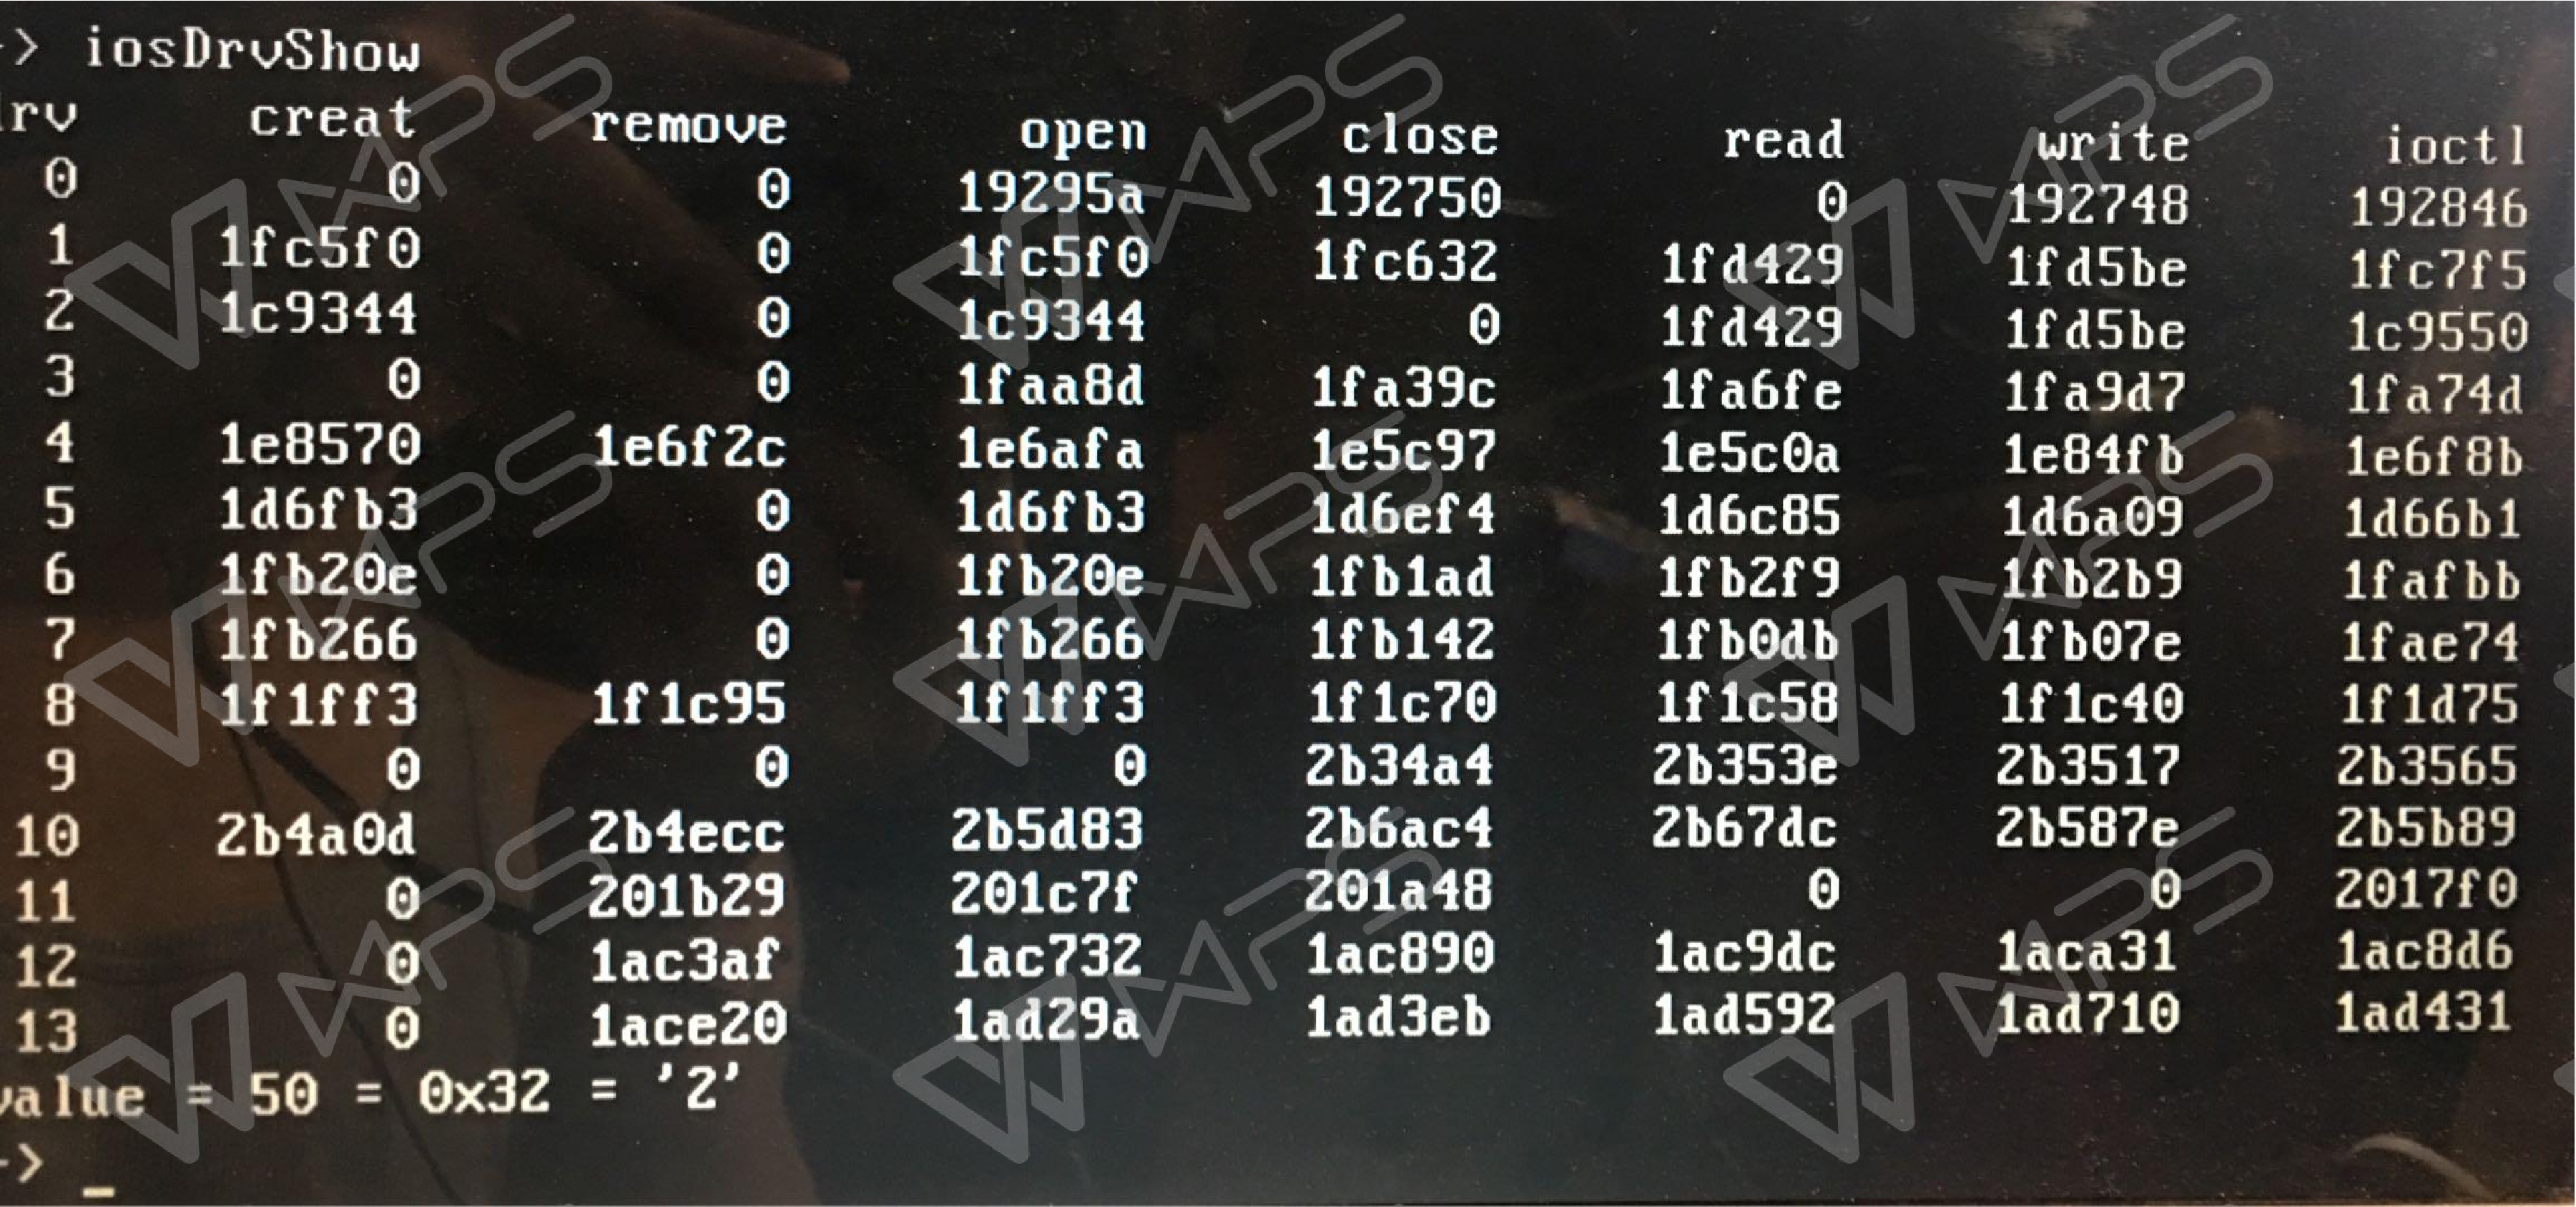
\includegraphics[width=.9\textwidth]{./graphics/iosDrvShow.pdf}
\caption{当前系统上的驱动表}\label{fig:iosDrvShow}
\end{figure}

\subsection{系统文件描述符表}
	系统描述符表存储着当前系统范围内打开的所有文件的描述符。文件描述符表底层实现上也是一个数组,正如设备驱动表表项索引用作驱动号,文件描述符表表项索引被用作文件描述符 ID,即 open 函数返回值。对于文件描述符有一点需要注意:标准输入,标准输出,标准错误输出虽然使用 0,1,2 三个文件描述符,但是可能在系统文件描述附表中只占用一个表项,即都使用同一个表项。Vxworks 内核将 0,1,2 三个标准文件描述符与系统文件描述符表中内容分开进行管理。实际上系统文件描述符中的内容更多的是针对硬件设备,即使用一次 open 函数调用就占用一个表项。0,1,2 三个标准文件描述符虽然占用 ID 空间(即其他描述符此时只能从 3 开始分配),但是其只使用了一次 open 函数调用,此后使用 ioGlobalStdSet 函数对 open 返回值进行了复制。
	
	系统文件描述符表中每个表项都是一个 FD\_ ENTRY 类型的结构,该结构定义在h/private/iosLibP.h 中,如下所示。
\lstset{language=C}
\begin{lstlisting}
typedef struct /* FD_ENTRY - entries in file table */ 
{ 
  DEV_HDR * pDevHdr;/* device header for this file */ 
  int value; /* driver's id for this file */ 
  char * name; /* actual file name */ 
  int taskId; /* task to receive SIGIO when enabled */ 
  BOOL inuse; /* active entry */ 
  BOOL obsolete; /* underlying driver has been deleted */ 
  void * auxValue;/* driver specific ptr, e.g. socket type */ 
  void * reserved; /* reserved for driver use */ 
} FD_ENTRY; 
\end{lstlisting}

用户程序每调用一次 open 函数,系统文件描述符表中就增加一个有效表项,直到数组满,此时 open函数调用将以失败返回。表项在表中的索引偏移 3 后作为文件描述符返回给用户,作为接下来其他所有操作的文件句柄。用户可以通过iosFdShow来显示系统文件描述符表中当前所有的有效表项,如\autoref{fig:iosFdShow}所示是当前系统下的文件系统描述符表。
\begin{figure}[!h]
\centering
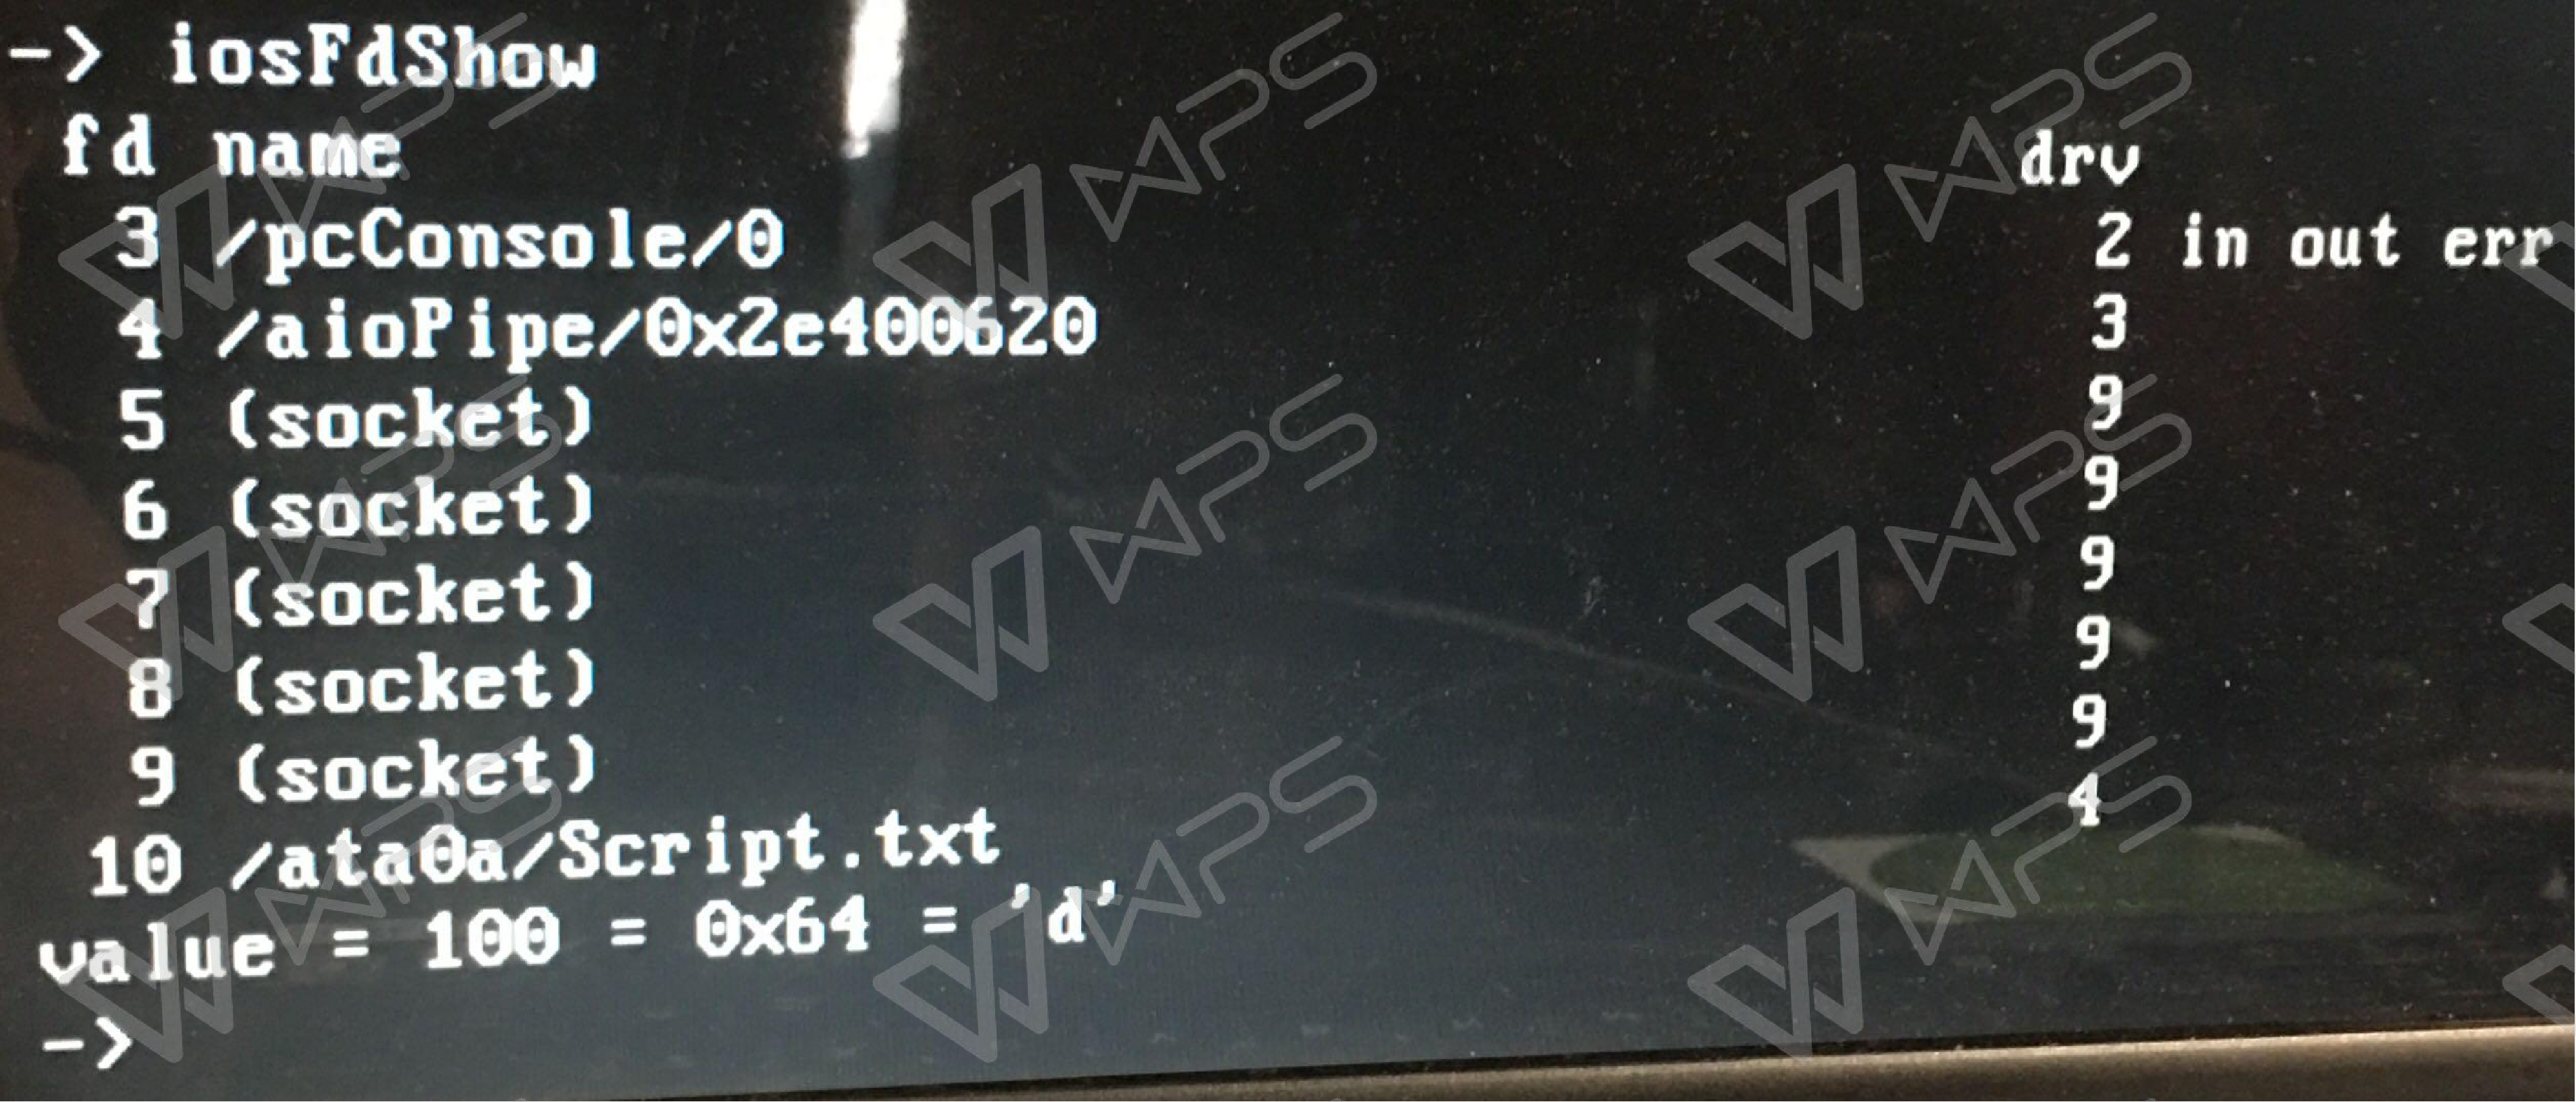
\includegraphics[width=.9\textwidth]{./graphics/iosFdShow.pdf}
\caption{当前系统上的文件描述符表}\label{fig:iosFdShow}
\end{figure}

\section{USB转串口设备驱动程序的实现}
	VxWorks调试通道当中运行的最主要的软件平台是嵌入式实时操作系统VxWorks,作为系统的最底层的软件,要想进行数据的传输,驱动程序是必不可少的。本系统中的硬件设备是基于USB总线的,USB口转串口设备的驱动程序在Windows和Linux下都有现成可用的,但是在VxWorks下需要自己来实现这部分。
	
\subsection{VxWorks上的USB协议栈}
	VxWorks的USB主机驱动程序堆栈满足USB协议规定的要求,提供了一整套服务来操作USB以及一些预置USB类驱动程序,以处理特定类型的USB设备。在Wind River的VxWorks中USB驱动程序堆栈的开发符合的是通用串行总线规范2.0版,USB系统是一种主从结构,系统的所有动作都是由USB主机发起,并协调不同的设备动作,设备端软件在系统中只需要对主机的命令做出响应即可,USB的主机端由于在系统中的地位比较特殊,因而其软件结构比较复杂,USB协议在主机端是分层实现的,其通信的逻辑结构和PC端的软硬件结构如\autoref{fig:usb通信结构}所示。USB协议由上至下可以分为三层:客户端驱动程序(Client Driver)、USB驱动(USBD)、主机控制器驱动(HCD),每一层完成不同的功能。

\begin{figure}[h]
\centering
  \begin{subfigure}[b]{0.4\textwidth}
  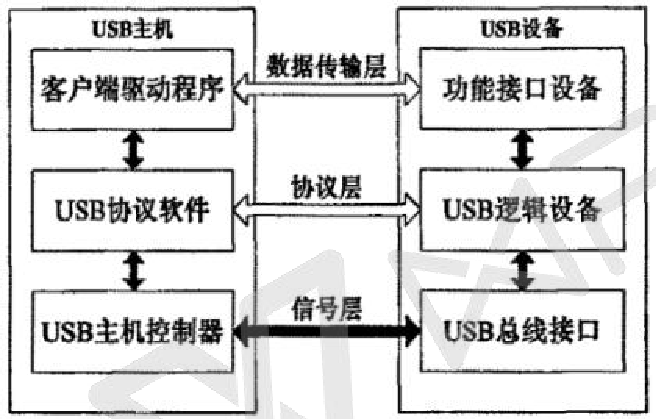
\includegraphics[width=1.0\textwidth]{./graphics/USB-device-structure-diagram.pdf}
  \caption{USB通信的逻辑结构}\label{fig:usb通信逻辑结构}
  \end{subfigure}
  ~
  \begin{subfigure}[b]{0.5\textwidth}
  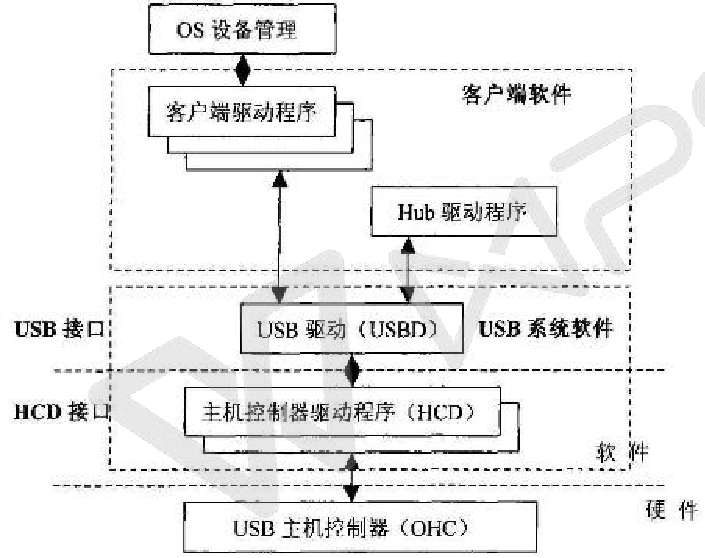
\includegraphics[width=1.0\textwidth]{./graphics/USB-PC-structure.pdf}
  \caption{USB主机端软硬件结构}\label{fig:usb-PC}
  \end{subfigure}
\caption{USB通信结构}\label{fig:USB通信结构}
\end{figure}
	
	客户端驱动程序完成对不同的设备类的设备的功能驱动。本次设计中所要完成的USB口转串口的驱动要完成的就是客户端驱动。为了和设备进行正常的通信,他通过USB的I/O请求包(I/O request,IRP)向USBD层发出数据接收或者发送的请求。此外,USB的传输机制对于客户端的驱动程序而言是完全透明的,客户端驱动程序所看到的仅仅是具体的设备类,不管设备采用的何种的数据传输方式。另外IRP是USB协议定义的抽象概念,其结构需要根据协议的具体来实现。
	
	USBD是USB的核心驱动,其提供的功能包括USB总线的枚举、总线带宽的分配、传输控制等操作。向上的接口负责处理客户端驱动程序提出的I/O请求,他通过IRP了解此设备的属性和本次数据通信的具体要求,将此IRP转换成USB能够识别的一系列的事物处理,交给HCD层或直接交给主机控制器处理。USBD还负责新设备的动态插拔、USB电源管理和对客户端驱动程序的维护等操作。
	
	HCD层的主要功能是与主机控制器合作完成USB的各种事物处理。它根据一定的规则调度所有奖杯广播发送到USB上的事物处理。调度方法是首先将数据传输类型组成不同的链表,每一种链表包括来自不同的设备驱动程序的同一种类型的数据,然后定义不同的数据类型在传输中所占的带宽比例,交给主机控制器处理,控制器根据规则从立案表上摘下数据块,根据大小为它创建一个或者多个事物处理,完成与设备的数据传输,当事物处理完成时HCD将结果交给USBD层。此外它还完成对主机控制器和根集线器的配置和驱动等操作。WindRiver提供了两种类型的主机控制器驱动:usbHcdUhciLib(UHCI主机控制器驱动)和usbHcdOhciLib(OHCI主机控制器驱动)。VxWorks的USBD和HCD之间的接口允许操过一个的底层主控制器,并且USBD能够同时连接多个USB HCD。这样的设计特点可以让开发者建立复杂的USB系统。

	在VxWorks系统当中UBSD层的驱动和HCD层的驱动都是已经实现好的,我们所需要实现的是客户端的驱动程序,用以驱动特定的USB设备。	


\subsection{特定需求单设备驱动的实现}

	由于对于仅支持单设备驱动程序是基于特定的需求而具体定制的,所以该设备的驱动程序的实现流程与通常的支持多设备的驱动的初始化流程存在差异。具体的需求为:
\hei{驱动中支持的设备名是固定的,驱动程序中要有缓存一定数据的能力,即使设备没有正确的连接也要能够往这个驱动中写入数据,并且一旦设备连接之后就能够将驱动中缓存的数据发送出去。}

	由于需要在设备未连接时就能够往设备中写入数据,且设备名为固定的,那么就必须调整驱动的初始化流程,使得其能够支持这一特性,通常驱动都是在设备加载之后再将其加入到系统设备表和系统驱动表当中,那么此时我们就需要先将一个固定的设备名加入到系统设备表当中。对于该特定需求的单设备驱动的流程图如\autoref{fig:single-usb-rs232drv-structure}所示。
\begin{figure}[!ht]
\centering
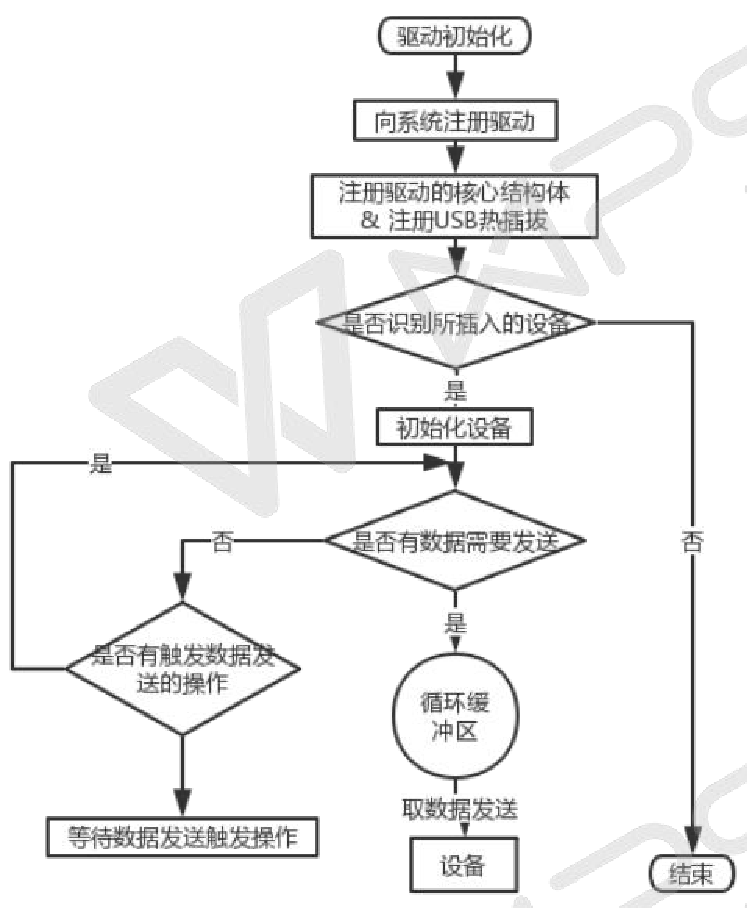
\includegraphics[width=.7\textwidth]{./graphics/sDevDrv.pdf}
\caption{特定需求的驱动流程图}\label{fig:single-usb-rs232drv-structure}
\end{figure}


\subsubsection{驱动的设备结构}
	底层驱动都要对其驱动的设备维护一个结构,用以保存设备的关键参数:USB配置、接口、端点地址、读写缓冲区的指针等等,这些信息将随着设备类型的不同而有所差别。对于我们此处要驱动的USB口转串口驱动,我们驱动中的关键数据结构如下: 
	
\lstset{language=C}
\begin{lstlisting}
typedef struct cp210x_dev
{
  DEV_HDR cp210xDevHdr; /*must be first field*/
  LINK 	devHdrLink;/*linked list of  devhdr structs*/
  UINT16                  numOpen;
  USBD_NODE_ID nodeId;			/*device nodeID*/
  UINT16 configuration;	/*configuration/interface reported as*/
  UINT16 interface;		/*a interface of this device*/
  UINT16 interfaceAltSetting;
  UINT16 vendorId;
  UINT16 productId;

  BOOL connected;
  USBD_PIPE_HANDLE outPipeHandle; /* USBD pipe handle for bulk OUT pipe */
  USB_IRP	outIrp;					/*IRP to monitor output to device*/
  BOOL outIrpInUse;
  UINT32 outErrors;				/*TRUE while IRP is outstanding*/
  UINT16  outEpAddr;	
  int trans_len;
  UINT8 trans_buf[64];
  
  USBD_PIPE_HANDLE inPipeHandle;
  USB_IRP inIrp;
  BOOL inIrpInUse;
  UINT8 inBuf[64];
  UINT32 inErrors;
  UINT16 	inEpAddr;
	
  char *writeBuf;
  int writeFront;
  int writeRear;
  char *readBuf;
  int readFront;
  int readRear;
} CP210X_DEV, *pCP210XDEV;
\end{lstlisting}
\noindent 部分成员的含义如下:

\begin{itemize}
\item DEV\_ HDR:自定义设备结构的第一个成员必须是DEV\_ HDR结构类型,对于内核的I/O子系统而言,其将所有的设备结构都看作是DEV\_ HDR类型,内核仅仅对DEV\_ HDR结构进行管理,在系统的设备列表中,内核只使用DEV\_ HDR结构当中的成员。自定义结构中的其他成员由驱动自己使用,内核并不了解这些自定义成员。
\item numOpen:用来记录设备被打开的次数,每次调用open()函数打开该设备则numOpen加一,调用close()函数关闭设备则减一。
\item nodeId:用来保存该设备在系统中的唯一ID号。
\item configure、interface、interfaceAltsetting:用来保存设备的描述符中的配置、接口、可变接口信息。
\item vendorId、productId:保存该设备的厂商ID和产品ID,用来识别该设备是否适合我们的驱动程序。
\item outPipeHandle、inPipeHandle:设备的输入/输出端点的管道句柄,每次传输数据时都需要使用该句柄来表明数据传到的哪一个端点。
\end{itemize}

\subsubsection{驱动注册和设备创建} 
	
	底层驱动一般提供形如 xxxDrv 和 xxxDevCreate 之类的函数完成驱动注册和设备创建的工作。这些工作的完成一般是在内核启动过程中进行。对于此处的USB口转串口驱动我们定义cp210xDrvInit() 初始化函数,其主要完成驱动所需要的资源申请和系统的初始化,包括创建信号量、向系统注册驱动、创建设备、向USBD层注册。cp210xDevInit模块主要代码如下所示:
\lstset{language=C}
\begin{lstlisting}
STATUS cp210xDrvInit(void)
{
  ...
  if(OSS_MUTEX_CREATE(&cp210xWriteMutex) != OK || OSS_MUTEX_CREATE(&cp210xReadMutex) != OK || OSS_MUTEX_CREATE(&cp210xMutex) != OK || (blockReadSem = semBCreate(SEM_Q_FIFO, SEM_EMPTY)) == NULL )
  ... 	
  cp210xDrvNum = iosDrvInstall(NULL,NULL,cp210xDevOpen,cp210xDevClose,
			cp210xDevRead,cp210xDevWrite,cp210xDevIoctl);
  ...
  if( iosDevAdd(&pCp210xDev->cp210xDevHdr,CP210X_NAME,cp210xDrvNum) != OK)
  ...  
  if(usbdClientRegister (CP210X_CLIENT_NAME, &cp210xHandle) != OK)
  ...  
  if(usbdDynamicAttachRegister(cp210xHandle,USBD_NOTIFY_ALL,USBD_NOTIFY_ALL,USBD_NOTIFY_ALL,TRUE,(USBD_ATTACH_CALLBACK)cp210xAttachCallback)!= OK)
  ...
}
\end{lstlisting}\\

	驱动会在进入初始化的时候首先检查该驱动是否已经安装,若已经安装了则无需再次安装,直接退出即可,cp210xDrvInit()通常是在usrRoot(usrConfig.c)中调用,但是你也可以手动调用这个函数对该驱动进行初始化操作。然后会进行一些驱动所需要的全局资源的初始化,如信号量、全局变量、看门狗等,接着调用iosDrvInstall()函数安装驱动的I/O函数,将其添加到驱动表当中,在我们的USB口转串口驱动当中不需要实现delete函数和create函数,直接将其指针置为NULL即可。
	
	注册完成之后还要向系统将该驱动程序添加到IO子系统当中,添加成功后会在系统的设备列表中显示该命名为CP210X\_ NAME的设备(CP210X\_ NAME只是一个宏定义,设备名可以自己更改)。此处即是我们的驱动程序中的一个特殊的地方,在没有识别到设备之前就已经创建好设备文件,只不过此时该设备还只是一个“假”的,只有软件实现,没有硬件支撑,即使此时已经可以打开该设备,向该设备写入数据,但是也只是写入到了系统的缓冲区当中而已,数据并没有发送到任何的硬件上。在驱动的内部我们会建立一个循环缓冲区来接收上层程序写入的数据,若系统中没有USB口转串口的设备,那么所有的数据就只会写入到该循环缓冲区当中,当循环缓冲区中的数据已经满了之后,遵循先进先出的原则来覆盖数据。当USB口转串口设备连接上时,若循环缓冲区当中已经有数据存在,则会立即启动发送数据的过程,若没有数据,则什么也不做。循环缓冲区的结构/功能如\autoref{fig:recruit-buffer-diagram}所示。
\begin{figure}[!h]
\centering
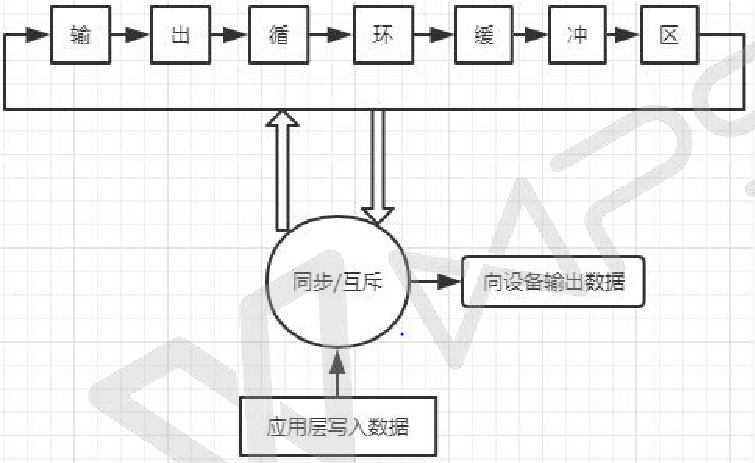
\includegraphics[width=.9\textwidth]{./graphics/recruit-buffer-diagram.pdf}
\caption{循环缓冲区结构/功能图}\label{fig:recruit-buffer-diagram}
\end{figure}

	接下来USB客户端驱动还需要向USBD层注册,注册完成之后会返回一个用于操作USBD的客户端handle,我们将其保存在cp210xHandle这个变量当中。然后还要注册一个动态注册的回调函数,当USBD层发现有USB设备的插拔动作时,就会根据我们注册时选定的设备类和接口类来判断是否需要调用我们注册的回调函数,由于我们的设备是一个特殊的设备,并不符合任何标准的USB设备类和接口类,于是我们将这两个参数置为USBD\_ NOTIFY\_ ALL,即任何USB设备的插拔都调用我们的注册的回调函数。之后我们在回调函数中根据设备的vendorId和productId来判断其是否是我们的驱动支持的设备,本驱动支持的设备的productId和vendorId存储在一个二维数组当中,判断过程是即遍历当前插入的设备的VID和PID是否在我们的数组当中。设备识别的流程如\autoref{fig:device-recognize}所示,目前支持的设备的设备ID、产品ID的组合如\autoref{tab:目前支持的设备列表}所示。

\begin{figure}[!h]
\centering
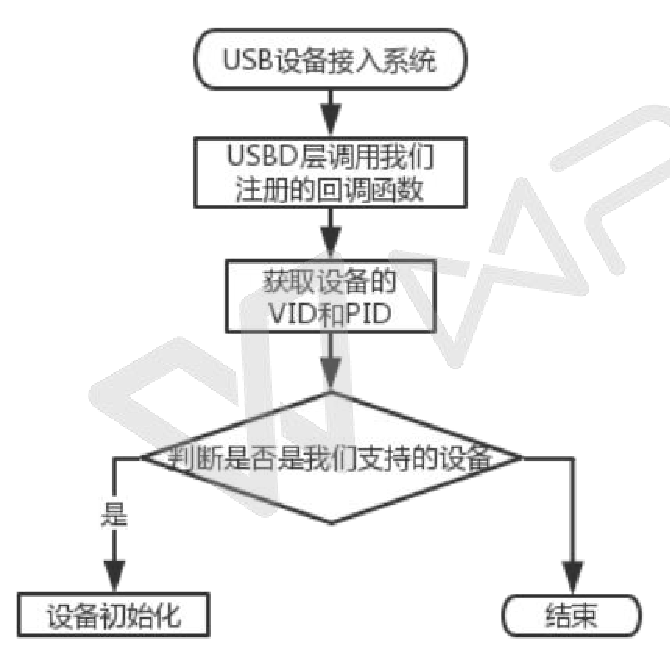
\includegraphics[width=.9\textwidth]{./graphics/device-recognize.pdf}
\caption{设备识别流程图}\label{fig:device-recognize}
\end{figure}


\begin{table}[!h]
\centering
\begin{tabular}{|c|c|c|c|c|c|c|}
\hline
{\hei{PID}}&{0x045B}&{0x0471}&{0x0489}&{0x0489}&{0x10C4}&{0x10C4}\\ 
\hline
{\hei{VID}}&{0x0053}&{0x066A}&{0xE000}&{0xE003}&{0x80F6}&{0x8115}\\
\hline 
{\hei{PID}}&{0x10C4}&{0x10C4}&{0x10C4}&{0x10C4}&{0x10C4}&{0x2405}\\
\hline
{\hei{VID}}&{0xEA60}&{0x813D}&{0x813F}&{0x814A}&{0x814B}&{0x0003}\\
\hline
\end{tabular}
\caption{目前支持的设备列表}\label{tab:目前支持的设备列表}
\end{table}

\subsubsection{设备的初始化}

设备的初始化包括获取该USB设备的各种描述符信息。包括设备描述符信息、配置描述符信息、接口描述符信息、端点描述符信息。再通过所获得的这些信息来创建到输出端点的管道和对设备进行设置,我们在此处将设备的波特率初始化为115200,数据位为8位,1个停止位,没有奇偶校验,没有流控。设备的初始化流程图如\autoref{fig:device-init}所示。

\begin{figure}[!h]
\centering
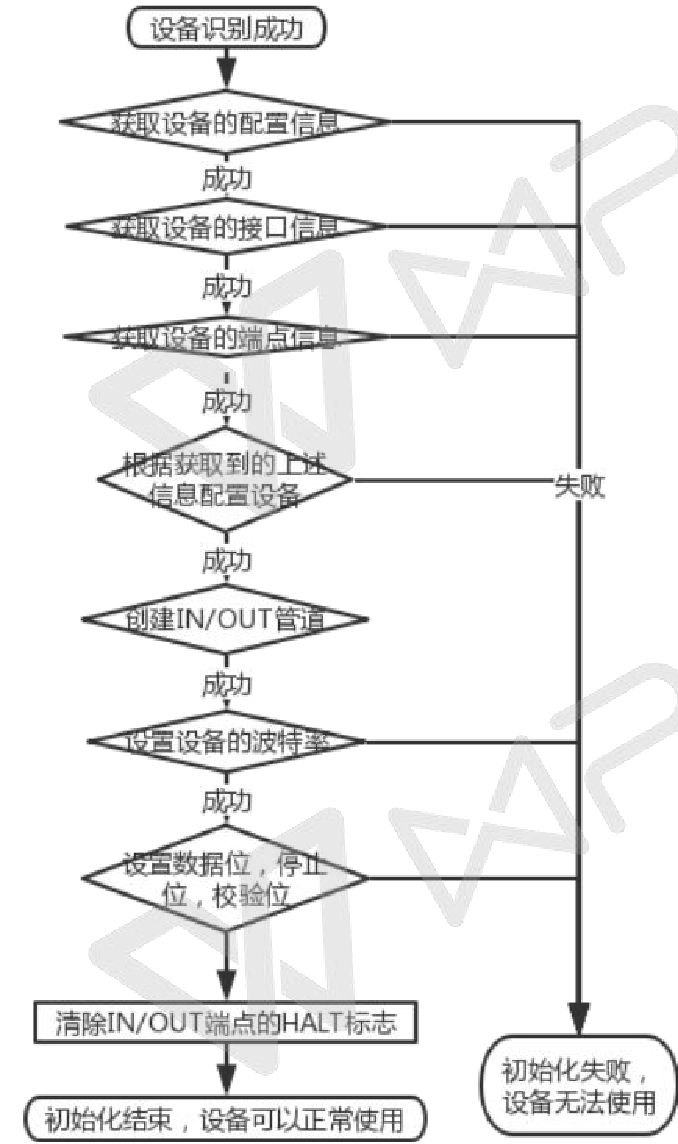
\includegraphics[width=.4\textwidth]{./graphics/device-init.pdf}
\caption{设备初始化流程图}\label{fig:device-init}
\end{figure}



\subsubsection{设备打开/关闭函数}

	用户在使用一个设备之前必须先打开这个设备,底层驱动响应函数中根据设备的需要将进行中断注册和使能设备工作配置等操作。对于我们的USB口转串口驱动而言,我们不需要自己管理中断,USBD层会为我们进行中断的管理工作,而配置工作我们在设备的初始化工作中已经完成,因此此处我们的设备打开工作,只需要简单的记录设备被打开的次数,并返回一个文件描述符即可。代码如下所示:
	
\lstset{language=C}
\begin{lstlisting}
LOCAL CP210X_DEV * cp210xDevOpen(DEV_HDR *pDevHdr, char *name, int flags,int mode)
{
	CP210X_DEV *pCp210xDev;
	pCp210xDev = (CP210X_DEV *)pDevHdr;
	(pCp210xDev->numOpen)++;
	return (pCp210xDev);
}
\end{lstlisting}


	需要注意的是第一个参数是由 IO 子系统提供的,IO 子系统在根据驱动号寻址到对应驱动函数时,其将系统设备列表中存储的设备结构作为第一个参数调用 cp210xDevOpen。实际上该参数是一个 CP210X\_ DEV 结构类型,但是 IO 子系统只认识DEV\_ HDR 结构。所以在 cp210xDevOpen函数中我们需要首先将这个 DEV\_ HDR 结构转换成 SPI\_ DEV,这基本上是所有底层驱动函数实现中第一条语句需要完成的任务。当然,驱动程序员也可以直接将第一个参数的类型设置为自定义结构类型,那么对于我们USB口转串口驱动,以上  cp210xDevOpen 函数的调用原型就变为:LOCAL int cp210xDevOpen(CP210X\_ DEV *pCp210xDev, char *name, int flags,int mode)这并不会造成什么影响,因为 IO 子系统传递过来实际上就是 CP210X\_ DEV 结构类型,只不过 IO 子系统对于驱动自定义参数并不关心,其只需要对 DEV\_ HDR 进行操作就可满足 IO 子系统本身管理的需要,其他自定义参数完全由底层驱动本身进行解释和使用。
	
	第二个参数是设备名匹配后的剩余部分,在我们的应用中,由于 open 函数调用时输入的路径名与系统设备列表中的设备名完全匹配,故此处的 name 应为空字符串。但是对于在文件系统层下的块设备而言,此处 name 指向的就是块设备节点名后的子目录和文件名。

	第三,四个参数就是用户 open 调用时传入的第二,三个参数,IO 子系统原封不动的将他们传递给了 cp210xDevOpen 函数。
	
	返回值为CP210X\_ DEV结构类型,一般返回如下两种值:一个有效的CP210X\_ DEV结构指针表示 cp210xDevOpen 调用成功,ERROR 则表示 cp210xDevOpen 调用失败,IO 子系统根据有效指针或者ERROR 返回一个文件描述符或者返回错误。cp210xDevOpen 函数的返回值非常重要,这个指针将被 IO 子系统保存,用于其后对驱动中读写,控制函数的调用。这个返回的指针将作为这些函数的第一个参数。
	
	设备的关闭和设备的打开操作是相反的操作,在关闭操作当中我们只需要对设备记录的打开次数进行减法操作即可。

\subsubsection{设备的读写}
	在成功打开一个设备后,用户程序将得到一个文件描述符,此后用户就可以使用这个文件描述符对设备进行读写,控制操作。底层驱动读写函数原型如下。

\lstset{language=C}
\begin{lstlisting}
LOCAL int cp210xDevWrite(CP210X_DEV *pCp210xDev, char *buffer,UINT32 nBytes)
LOCAL int cp210xDevRead(CP210X_DEV *pCp210xDev, char *buffer,UINT32 nBytes)
\end{lstlisting}

此处我们将这两个函数的第一个参数类型直接设置为 CP210X\_ DEV 结构类型而不是DEV\_ HDR,只是为了向大家展示两种方式都是允许的,在我们的实际编程中应该一种方式一以贯之。cp210xDevWrite,cp210xDevRead函数的第一个参数是实际上是cp210xDevOpen 函数的返回值。

由于我们的驱动程序的初始化方式比较特殊,所以此处对数据的输出操作的流程也需要有相应的改变。在驱动程序中我们设置了一个4K的数据缓冲区来接收数据,设备的初始化之后就先查询缓冲区中是否存在数据,若存在数据则将其发送,若不存在则等待其他程序调用write写入数据来触发数据的发送操作,系统调用write()在该驱动程序中对应的函数为cp210xDevWrite()函数,这个函数会接受write()发送过来的数据,并将其存入缓冲区中,并判断是否需要触发数据的发送操作。发送数据的触发操作只会在当前没有数据在发送时完成,若调用write时设备已经在发送数据,则只是将write的数据存入缓冲区,设备发送完当前正在发送的数据之后会去判断缓冲区中是否还有数据,有数据则会继续发送。其流程图如\autoref{fig:outData-diagram} 所示。

\begin{figure}[!h]
\centering
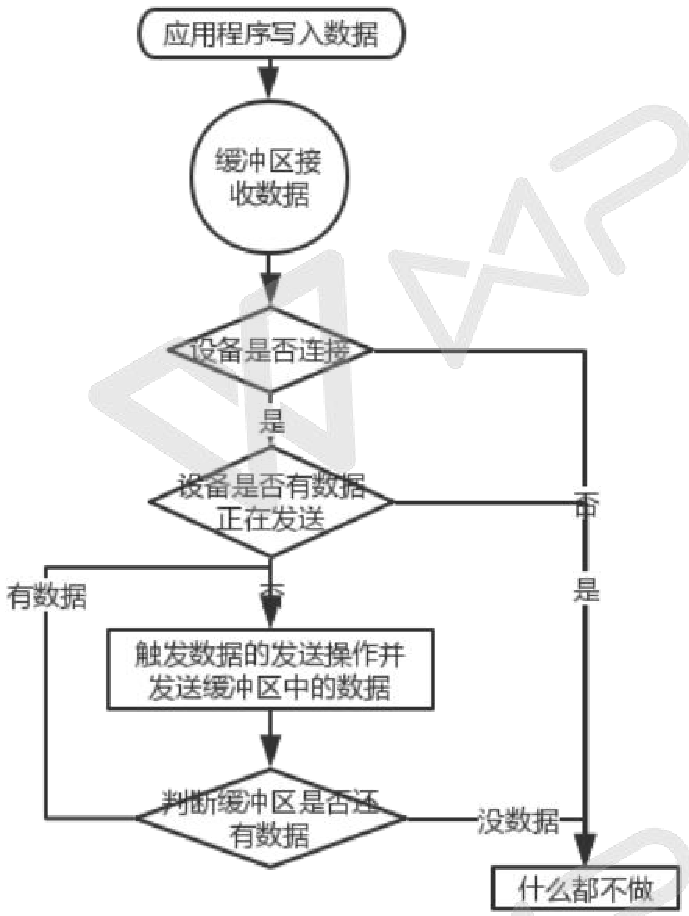
\includegraphics[width=.4\textwidth]{./graphics/outData-diagram.pdf}
\caption{数据发送逻辑图}\label{fig:outData-diagram}
\end{figure}

cp210xDevRead 和 cp210xDevWrite 的实现非常相似,只是更换了一下数据的传输方向。cp210xDevRead在底层也有一个循环缓冲区用来接收从USB口转串口设备发送来的数据,当需要读取 nbytes 个字节而缓冲区内的字节不够时,read就会阻塞,直到USBD层通知你有新的数据到来时才会继续进行读操作。同时也在驱动中启动了一个计时器,如果在计时器时间到了之后,还未能满足需要读取的字节数,则退出本次读写操作,返回当前已处理的字节数。


\subsubsection{设备的控制操作}
	设备控制简单的说用户对于设备某些工作行为的再配置。基于设备的类型,这些由驱动和 IO 子系统提供给用户的再配置参数会有所差别。Vxworks(其他通用操作系统也是如此)对各种类型的设备都抽取了一组共同属性作为配置选项,如串口波特率再配置就是一个串口标准属性。事实上,虽然有所约定,底层驱动完成可以虽然有所约定,底层驱动完成可以按照自己的标准对这些再配置属性进行选择:可以选择只实现其中某些再配置参数,可以按照特定设备的特殊情况选择对某个再配
置选项的响应方式或者转移再配置参数等等。可以说,设备控制函数既提供给了用户控制设备的方便性,也对底层设备的实现提供了极大的方便性,当然,底层驱动程序员不可以“欺骗”用户,必须完成用户要求的基本配置要求方可根据需要在做一些辅助性的配置工作,这是底层驱动设备控制实现函数的基本原则。

	除了 Vxworks 操作系统本身提供的控制参数外,对于一个特定设备也有自己的特定参数,这些也可以作为选项提供给用户进行控制。一般而言,底层驱动需要定义一个头文件,将设备特定参数在其中进行定义,而后将这个头文件提供给用户程序,当用户对设备进行操作时,其包含这个头文件,使用其中定义的特定参数对设备进行控制。IO 子系统实际上不加任何
改变的将用户使用的选项参数或者控制命令传递给了底层驱动,由底层驱动完成对选项参数或控制命令的解释和使用。
设备控制函数原型如下:
\lstset{language=C}
\begin{lstlisting}
LOCAL int cp210xDevIoctl(CP210X_DEV *pCp210xDev, int request, void *someArg )
\end{lstlisting}

对于我们的 USB口转串口S驱动,在实际使用中,再配置参数和命令有很多,但是目前我们只提供设备的波特率、数据位、校验位、流控的参数和命令。


\subsubsection{驱动卸载}
	在驱动的初始化中我们使用 iosDrvInstall 函数向 IO 子系统注册了我们的驱动,同时 IO 子系统也提供了另外一个相反作用的函数注销我们的驱动,这个函数就是 iosDrvRemove。该函数调用原型如下 :
\lstset{language=C}
\begin{lstlisting}
STATUS iosDrvRemove 
 ( 
 int drvnum, /* driver to remove, returned by iosDrvInstall()*/ 
 BOOL forceClose /* if TRUE, force closure of open files */ 
); 
\end{lstlisting}

该函数的第二个参数指定是否强制进行卸载,并将所有与此驱动有关的文件描述符关闭。如果强制关闭,则 IO 子系统将遍历系统文件描述符表,检查每个描述符对应结构中的驱动号是否等于要卸载驱动的驱动号,如果相同,则调用这个驱动的 close 实现函数进行关闭,同时释放文件描述符表中该表项,此时用户层的文件句柄将自动失去功效,如果用户其后使用这个文件描述符,将直接得到一个错误返回。

除了驱动卸载函数之外,我们的驱动初始化时还向USBD层进行了注册,在卸载的时候也应该注销USBD层的注册,同时注销动态注册的回调函数并从系统的设备表当中删除掉该设备。之后还应该对该驱动占用的所有其他的系统资源进行释放。



至此,我们已经完成了该特定需求下的USB口转串口驱动程序的所有组成部分的设计和实现。

\subsection{通用多设备驱动的实现}



%\subsection{第二层}\label{sec:1}
%\subsubsection{第三层}\label{sec:1}
%测试测试测试测试测试测试测试测试测试测试测试测试。
%\footnote{\label{footnote:1}脚注}

\section{字体}

普通\textbf{粗体}\emph{斜体}

\hei{黑体}\kai{楷体}\fangsong{仿宋}

\section{公式}

单个公式,公式引用:\autoref{eq:1}。
\begin{equation}
 c^2 = a^2 + b^2 \label{eq:1}
\end{equation}

多个公式,公式引用:\autoref{eq:2},\autoref{eq:3}。

\begin{subequations}
\begin{equation}
  F = ma \label{eq:2}
\end{equation}
\begin{equation}
  E = mc^2 \label{eq:3}
\end{equation}
\end{subequations}

\section{罗列环境}

\begin{enumerate}
    \item 第一层\label{item:1}
    \item 第一层
    \begin{enumerate}
        \item 第二层\label{item:2}
        \item 第二层
        \begin{enumerate}
            \item 第三层\label{item:3}
            \item 第三层
        \end{enumerate}
    \end{enumerate}
\end{enumerate}

\begin{description}
    \item[解释环境]  解释内容
\end{description}



\clearpage

\section{代码环境}

\begin{lstlisting}[language=python]
import os

def main():
    '''
    doc here
    '''
    print 'hello, world' # Abc
    print 'hello, 中文' # 中文
\end{lstlisting}

\section{定律证明环境}

\begin{definition}\label{def:1}
这是一个定义。
\end{definition}
\begin{proposition}\label{proposition:1}
这是一个命题。
\end{proposition}
\begin{axiom}\label{axiom:1}
这是一个公理。
\end{axiom}
\begin{lemma}\label{lemma:1}
这是一个引理。
\end{lemma}
\begin{theorem}\label{theorem:1}
这是一个定理。
\end{theorem}
\begin{proof}\label{proof:1}
这是一个证明。
\end{proof}

\section{算法环境}

\begin{algorithm}[H]
\SetAlgoLined
\KwData{this text}
\KwResult{how to write algorithm with \LaTeX2e }
initialization\;\label{alg_line:1}
\While{not at end of this document}{
read current\;
\eIf{understand}{
go to next section\;
current section becomes this
 one\;
}{
go back to the beginning of current section\;
}
}
\caption{How to write algorithms}\label{alg:1}
\end{algorithm}

\section{表格}
表格见\autoref{tab:1}。

\begin{table}[!h]
\centering
\caption{一个表格}\label{tab:1}
\begin{tabular}{|c|c|}
\hline
a & b \\
\hline
c & d \\
\hline
\end{tabular}
\end{table}
\section{图片}
图片见\autoref{fig:1}。图片格式支持eps,png,pdf等。多个图片见\autoref{fig:2},分开引用:\autoref{fig:2-1},\autoref{fig:2-2}。

\begin{figure}[!h]
\centering

\includegraphics[width=.4\textwidth]{hust-title.pdf}
\caption{hust-title}\label{fig:hust-title}
\end{figure}

\begin{figure}[!h]
\centering
  \begin{subfigure}[b]{0.3\textwidth}
  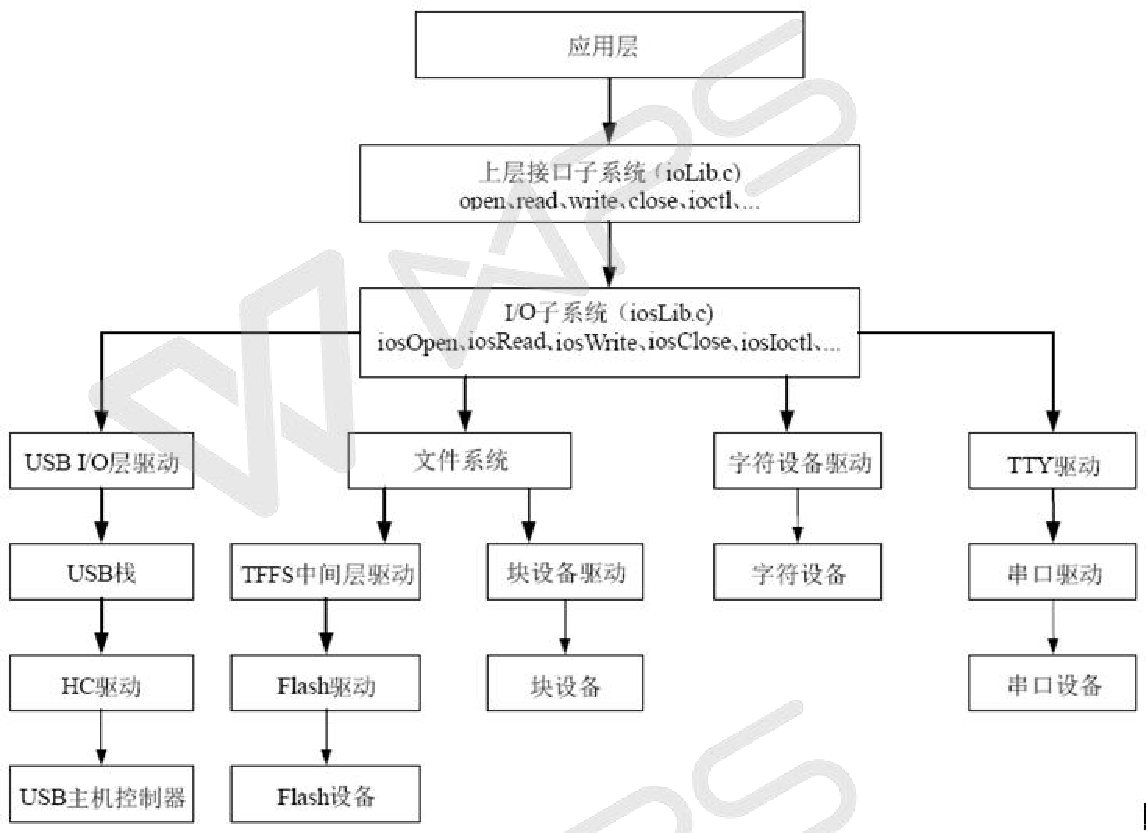
\includegraphics[width=\textwidth]{./data/VxWorks-driver-structure.pdf}
  \caption{VxWorks-driver-structure}\label{fig:2-1}
  \end{subfigure}
  ~
  \begin{subfigure}[b]{0.3\textwidth}
  \includegraphics[width=\textwidth]{fig-example.pdf}
  \caption{图片2}\label{fig:2-2}
  \end{subfigure}
\caption{多个图片}\label{fig:2}
\end{figure}

\section{参考文献示例}
这是一篇中文参考文献\cite{徐媛媛2003嵌入式实时操作系统的设备驱动};这是一篇英文参考文献\cite{9787508342894};同时引用\cite{9780124467422,bamboosilk}。

\section[\textbackslash{}autoref 测试]{\texttt{\textbackslash{}autoref} 测试}

\begin{description}
  \item[公式] \autoref{eq:1}
  \item[脚注] \autoref{footnote:1}
  \item[项] \autoref{item:1},\autoref{item:2},\autoref{item:3}
  \item[图] \autoref{fig:1}
  \item[表] \autoref{tab:1}
  \item[附录] \autoref{appendix:1}
  \item[章] \autoref{chapter:1}
  \item[小节] \autoref{sec:1},\autoref{sec:2},\autoref{sec:3}
  \item[算法] \autoref{alg:1},\autoref{alg_line:1}
  \item[证明环境] \autoref{def:1},\autoref{proposition:1},\autoref{axiom:1},\autoref{lemma:1},\autoref{theorem:1},\autoref{proof:1}
\end{description}

% backmatter用于表示论文的正文结束
\backmatter

%ack 环境用于致谢页面
\begin{ack}
致谢正文。
\end{ack}

% bibliography用于生成参考文献。
\bibliography{ref/myref.bib}

% appendix环境用于附录环境。即可以将附录置于appendix环境当中。如:
% \begin{appendix}
%  <content>
% \end{appendix}

% 直接使用\appendix 则表明后文均为附录。如:
% \appendix
%  <content> 
\appendix

% publications环境用于已经发表了的论文的页面,一般用于附录当中,使用上同enumerate环境
\begin{publications}
    \item 论文1
    \item 论文2
\end{publications}

\chapter{这是一个附录}\label{appendix:1}
附录正文。


\end{document}

\endinput
%%
%% End of file `hustthesis-zh-example.tex'.
